% Options for packages loaded elsewhere
\PassOptionsToPackage{unicode}{hyperref}
\PassOptionsToPackage{hyphens}{url}
%
\documentclass[
  a4paper,
]{scrbook}

\usepackage{amsmath,amssymb}
\usepackage{lmodern}
\usepackage{iftex}
\ifPDFTeX
  \usepackage[T1]{fontenc}
  \usepackage[utf8]{inputenc}
  \usepackage{textcomp} % provide euro and other symbols
\else % if luatex or xetex
  \usepackage{unicode-math}
  \defaultfontfeatures{Scale=MatchLowercase}
  \defaultfontfeatures[\rmfamily]{Ligatures=TeX,Scale=1}
  \setmainfont[]{Latin Modern Roman}
  \setsansfont[]{Latin Modern Roman}
\fi
% Use upquote if available, for straight quotes in verbatim environments
\IfFileExists{upquote.sty}{\usepackage{upquote}}{}
\IfFileExists{microtype.sty}{% use microtype if available
  \usepackage[]{microtype}
  \UseMicrotypeSet[protrusion]{basicmath} % disable protrusion for tt fonts
}{}
\makeatletter
\@ifundefined{KOMAClassName}{% if non-KOMA class
  \IfFileExists{parskip.sty}{%
    \usepackage{parskip}
  }{% else
    \setlength{\parindent}{0pt}
    \setlength{\parskip}{6pt plus 2pt minus 1pt}}
}{% if KOMA class
  \KOMAoptions{parskip=half}}
\makeatother
\usepackage{xcolor}
\setlength{\emergencystretch}{3em} % prevent overfull lines
\setcounter{secnumdepth}{5}
% Make \paragraph and \subparagraph free-standing
\ifx\paragraph\undefined\else
  \let\oldparagraph\paragraph
  \renewcommand{\paragraph}[1]{\oldparagraph{#1}\mbox{}}
\fi
\ifx\subparagraph\undefined\else
  \let\oldsubparagraph\subparagraph
  \renewcommand{\subparagraph}[1]{\oldsubparagraph{#1}\mbox{}}
\fi


\providecommand{\tightlist}{%
  \setlength{\itemsep}{0pt}\setlength{\parskip}{0pt}}\usepackage{longtable,booktabs,array}
\usepackage{calc} % for calculating minipage widths
% Correct order of tables after \paragraph or \subparagraph
\usepackage{etoolbox}
\makeatletter
\patchcmd\longtable{\par}{\if@noskipsec\mbox{}\fi\par}{}{}
\makeatother
% Allow footnotes in longtable head/foot
\IfFileExists{footnotehyper.sty}{\usepackage{footnotehyper}}{\usepackage{footnote}}
\makesavenoteenv{longtable}
\usepackage{graphicx}
\makeatletter
\def\maxwidth{\ifdim\Gin@nat@width>\linewidth\linewidth\else\Gin@nat@width\fi}
\def\maxheight{\ifdim\Gin@nat@height>\textheight\textheight\else\Gin@nat@height\fi}
\makeatother
% Scale images if necessary, so that they will not overflow the page
% margins by default, and it is still possible to overwrite the defaults
% using explicit options in \includegraphics[width, height, ...]{}
\setkeys{Gin}{width=\maxwidth,height=\maxheight,keepaspectratio}
% Set default figure placement to htbp
\makeatletter
\def\fps@figure{htbp}
\makeatother

\usepackage{titling}
\setlength{\droptitle}{-2cm}
\preauthor{
  \begin{center}
  \Large
  \vspace{10mm}
  by

  \vspace{20mm}
}
\postauthor{
  \end{center}
  \vfill
}

\predate{
  \begin{center}
  A thesis 
  submitted in fulfilment of the \\
  requirements of the degree of \\
  Doctor of Philosophy in Physics\\               % Degree
  School of Physical and Chemical Sciences\\          % Department
  Te Herenga Waka - Victoria University of Wellington\\                       % University 
  \vspace{5mm}
}
\postdate{
  \\
  
\includegraphics[width=3in,height=1.5in]{figures/VUW-logo.png}\\
  \end{center}
  }
\makeatletter
\makeatother
\makeatletter
\@ifpackageloaded{bookmark}{}{\usepackage{bookmark}}
\makeatother
\makeatletter
\@ifpackageloaded{caption}{}{\usepackage{caption}}
\AtBeginDocument{%
\ifdefined\contentsname
  \renewcommand*\contentsname{Table of contents}
\else
  \newcommand\contentsname{Table of contents}
\fi
\ifdefined\listfigurename
  \renewcommand*\listfigurename{List of Figures}
\else
  \newcommand\listfigurename{List of Figures}
\fi
\ifdefined\listtablename
  \renewcommand*\listtablename{List of Tables}
\else
  \newcommand\listtablename{List of Tables}
\fi
\ifdefined\figurename
  \renewcommand*\figurename{Figure}
\else
  \newcommand\figurename{Figure}
\fi
\ifdefined\tablename
  \renewcommand*\tablename{Table}
\else
  \newcommand\tablename{Table}
\fi
}
\@ifpackageloaded{float}{}{\usepackage{float}}
\floatstyle{ruled}
\@ifundefined{c@chapter}{\newfloat{codelisting}{h}{lop}}{\newfloat{codelisting}{h}{lop}[chapter]}
\floatname{codelisting}{Listing}
\newcommand*\listoflistings{\listof{codelisting}{List of Listings}}
\makeatother
\makeatletter
\@ifpackageloaded{caption}{}{\usepackage{caption}}
\@ifpackageloaded{subcaption}{}{\usepackage{subcaption}}
\makeatother
\makeatletter
\@ifpackageloaded{tcolorbox}{}{\usepackage[many]{tcolorbox}}
\makeatother
\makeatletter
\@ifundefined{shadecolor}{\definecolor{shadecolor}{rgb}{.97, .97, .97}}
\makeatother
\makeatletter
\makeatother
\ifLuaTeX
  \usepackage{selnolig}  % disable illegal ligatures
\fi
\usepackage[citestyle = ieee,urldate = iso8601]{biblatex}
\addbibresource{references.bib}
\IfFileExists{bookmark.sty}{\usepackage{bookmark}}{\usepackage{hyperref}}
\IfFileExists{xurl.sty}{\usepackage{xurl}}{} % add URL line breaks if available
\urlstyle{same} % disable monospaced font for URLs
\hypersetup{
  pdftitle={Volatile Organic Compound Detection Using Insect Odorant-Receptor Functionalised Field-Effect Transistors},
  pdfauthor={Eddyn Oswald Perkins Treacher},
  hidelinks,
  pdfcreator={LaTeX via pandoc}}

\title{Volatile Organic Compound Detection Using Insect Odorant-Receptor
Functionalised Field-Effect Transistors}
\author{Eddyn Oswald Perkins Treacher}
\date{Oct 2023}

\begin{document}
\frontmatter
\maketitle
\ifdefined\Shaded\renewenvironment{Shaded}{\begin{tcolorbox}[interior hidden, breakable, borderline west={3pt}{0pt}{shadecolor}, sharp corners, boxrule=0pt, enhanced, frame hidden]}{\end{tcolorbox}}\fi

\mainmatter
\bookmarksetup{startatroot}

\hypertarget{acknowledgements}{%
\chapter*{Acknowledgements}\label{acknowledgements}}
\addcontentsline{toc}{chapter}{Acknowledgements}

\markboth{Acknowledgements}{Acknowledgements}

\begin{verbatim}
69450
\end{verbatim}

Rifat, Alex - vapour sensor Erica Cassie - FET sensing setup Rob Keyzers
and Jennie Ramirez-Garcia - NMR spectra Patricia Hunt - Computational
chemistry

\bookmarksetup{startatroot}

\hypertarget{sec-fabrication}{%
\chapter{Fabrication of Carbon Nanotube Network and Graphene
Field-Effect Transistors}\label{sec-fabrication}}

This chapter discusses the fabrication processes for both the carbon
nanotube network and graphene field-effect transistors (FETs).
Experimental optimisation of the transducer element is critical for
biosensor work, and large numbers of transducers were required for
testing various biosensor functionalisation processes. Therefore, these
processes were developed to rapidly fabricate devices with reproducible
device characteristics appropriate for biosensing work. Also outlined in
this chapter are the characterisation techniques taken to test the
quality and reproducibility of these fabrication processes.

The nitrogen (\(\geq\) 99.99\%) and oxygen (99.7\%) used in fabrication
work was supplied by BOC Limited New Zealand. All acetone and
isopropanol used for wafer/device processing had a minimum 99.9\% purity
(HPLC grade). Deionised (DI) water was taken from a
Synergy\(^\circledR\) UV Water Purification System. The DI water had a
measured conductivity of
\((1.4\pm0.1)\textrm{ } \mu \textrm{S cm}^{-1}\), compared to tap water
with a measured conductivity of
\((7.8\pm0.2)\textrm{ } \mu \textrm{S cm}^{-1}\).

\hypertarget{sec-photolithography}{%
\section{Photolithography for Carbon Nanotube and Graphene Field-Effect
Transistors}\label{sec-photolithography}}

\begin{figure}

{\centering 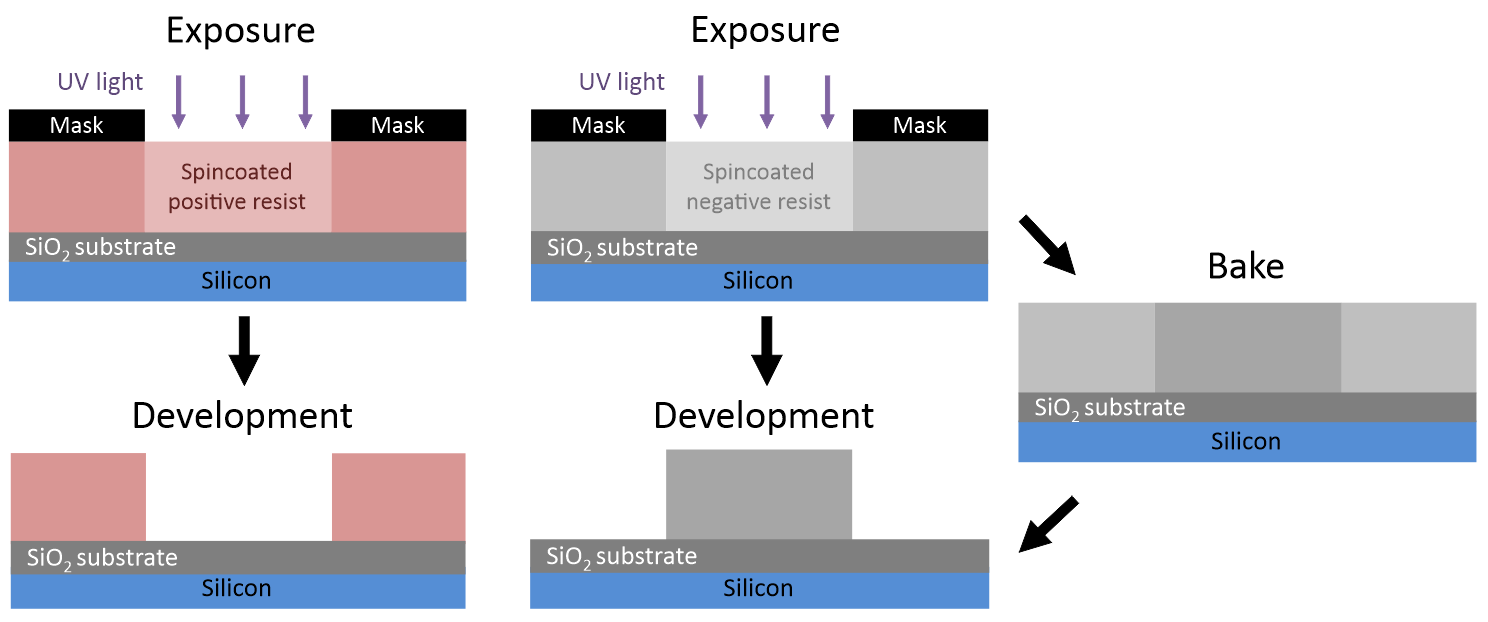
\includegraphics{./figures/ch4/positive-negative-photolithography.png}

}

\caption{\label{fig-photolithography-types}A side-view comparison of
generic photolithography processes for positive and negative resists in
the ideal case. Photolithography with a positive resist requires a
single softbake step before exposure, while for negative resists a
second baking step is required after exposure (Thicknesses shown not to
scale).}

\end{figure}

This section details some of the standard photolithography procedures
used in the quarter wafer processing detailed in
Section~\ref{sec-qw-processing}. Photoresists, also referred to here as
``resists'', are UV light-sensitive polymeric resins used for
photolithography. Both positive and negative photoresists were used in
various fabrication processes. Positive resists are made soluble in
alkalines by UV light exposure, meaning exposed areas are removed in the
development process. Conversely, negative resists are cross-linked by
exposure and a post-exposure bake step. The unexposed areas of the
negative resist are then removed in the development process
\autocite{Microchemicals}. Figure~\ref{fig-photolithography-types} gives
a visual representation of these differences.

The specific photoresist selected for photolithography depends on the
specific use case. The types used in this thesis are positive and
negative AZ\(^\circledR\) photoresists (AZ\(^\circledR\) 1518,
Microchemicals GmbH; AZ\(^\circledR\) nLOF 2020, Microchemicals GmbH)
and SU-8 (SU8-2150, Kayaku Advanced Materials, formerly Microchem). The
AZ\(^\circledR\) resists used here have a minimum film thickness of
\(1.5\textrm{ } \mu \textrm{m}\) \autocite{Microchemicals}, while the
SU8-2150 has a minimum film thickness of
\(0.5\textrm{ } \mu \textrm{m}\) \autocite{Kayaku}. Positive resists
which have not been thermally crosslinked will soften at higher
temperatures (\(\gtrsim 100^\circ\)C for AZ\(^\circledR\) 1518), leading
to a rounded profile. This is not the case for negative resists, which
are more thermally stable \autocite{Microchemicals}. Each resist
therefore has a different cross-section profile, as shown in
Figure~\ref{fig-photolithography-profiles}.

\begin{figure}

\begin{minipage}[t]{0.47\linewidth}

{\centering 

\raisebox{-\height}{

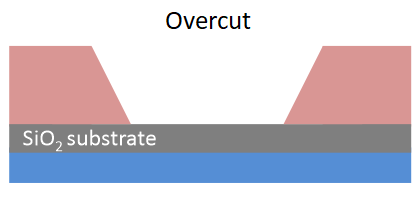
\includegraphics{./figures/ch4/overcut-profile.png}

}

}

\subcaption{\label{fig-overcut-profile}}
\end{minipage}%
%
\begin{minipage}[t]{0.05\linewidth}

{\centering 

~

}

\end{minipage}%
%
\begin{minipage}[t]{0.47\linewidth}

{\centering 

\raisebox{-\height}{

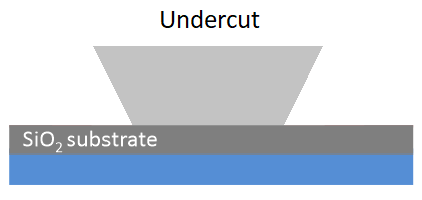
\includegraphics{./figures/ch4/undercut-profile.png}

}

}

\subcaption{\label{fig-undercut-profile}}
\end{minipage}%

\caption{\label{fig-photolithography-profiles}The overcut profile of a
positive resist pattern is shown in (a). The undercut profile in (b) is
ideal for thin-film metal deposition and subsequent patterned removal,
known as ``lift-off''. Each profile has had the central region of the
substrate exposed to UV light prior to development.}

\end{figure}

If metal deposition is performed on a positive resist, some metal can
collect on the outwardly-sloped sidewalls of the resist (see
Figure~\ref{fig-photolithography-profiles}) which forms significant
spikes on the edges of the deposited metal upon lift-off. On the other
hand, metal cannot collect on top of the inwardly-sloped negative
profile sidewalls, which avoids the formation of large edge spikes.
Therefore, the negative resist profile is more suited to metal or metal
oxide deposition and lift-off processes, though the process is more
sensitive to human error due to requiring more processing steps than
positive resist \autocite{Microchemicals}. Finally, when it is suitably
processed SU-8 is considered to be more stable and biocompatible than
other photoresists \autocite{Albarghouthi2022}. It is especially
biocompatible when chemically modified via processes such as isopropanol
sonication and O\(_2\) plasma treatment \autocite{Chen2021}.

All photolithographic exposure was performed using a Karl Suss MJB3
Contact Aligner with a USHIO super-high pressure 350 W mercury lamp
(USH-350DS, Japan). When performing photolithography, the intensity
reading from the aligner was \(20.8-24.2\) mW/cm\(^2\) (Note however
that an external photometer reading at 400 nm found an intensity output
of 17.2 mW/cm\(^2\) when the aligner read 21.0 mW/cm\(^2\)).

In general, photolithography procedures should be performed under yellow
lighting, as light wavelengths from \(320-450\) nm can promote reactions
in the photoresist used. Aging of photoresist over time can also
significantly affect the photolithography process, and therefore all
processes should be re-optimised regularly over time to give the desired
result \autocite{Microchemicals}. The range in processing times for some
steps of the processes used here are largely due to the effects of aging
on the photoresist.

The step-by-step processes for each resist are detailed in the
subsequent sections.

\hypertarget{azcircledr-1518-photoresist}{%
\subsection{\texorpdfstring{AZ\(^\circledR\) 1518
photoresist}{AZ\^{}\textbackslash circledR 1518 photoresist}}\label{azcircledr-1518-photoresist}}

\begin{enumerate}
\def\labelenumi{\arabic{enumi}.}
\item
  Spincoat at a final speed of 4000 rotations per minute (rpm) for 1
  minute, with an initial acceleration of 500 rpm/s (notes: clean the
  substrate with acetone, isopropanol (IPA) and nitrogen before
  spincoating; use only the minimum amount of photoresist required to
  fully cover the wafer surface; avoid any gaps or bubbles in the
  photoresist).
\item
  Softbake \(2-4\) minutes at \(95^\circ\)C on the hotplate (2 min for
  individual devices, 4 min for a quarter wafer)
\item
  Mask expose for \(10-12\) s (note: clean mask with acetone/IPA and
  N\(_2\) dry before use)
\item
  Develop with 3 parts AZ\(^\circledR\) 326 (2.38 \% TMAH metal-ion free
  developer, Microchemicals GmbH) in 1 part deionised (DI) water for
  \(30-45\) s (note: rinse for \(10-15\) s in one development solution,
  then perform the rest of the development in clean developer for a
  cleaner profile; lightly agitate the solution throughout the
  development process)
\item
  Rinse device for 30 s in DI water to remove excess developer, then dry
  under nitrogen
\end{enumerate}

\hypertarget{azcircledr-nlof-2020-photoresist}{%
\subsection{\texorpdfstring{AZ\(^\circledR\) nLOF 2020
photoresist}{AZ\^{}\textbackslash circledR nLOF 2020 photoresist}}\label{azcircledr-nlof-2020-photoresist}}

\begin{enumerate}
\def\labelenumi{\arabic{enumi}.}
\item
  Spincoat at final speed of 3000 rotations per minute (rpm) for 1
  minute, with an initial acceleration of 500 rpm/s (notes: clean the
  substrate with acetone, isopropanol (IPA) and nitrogen before
  spincoating; avoid any gaps or bubbles in the photoresist)
\item
  Softbake for precisely 60 s at \(110^\circ\)C on the hotplate
\item
  Mask expose for \(2.7-3\) s (note: clean mask with acetone/IPA and
  N\(_2\) dry before use)
\item
  Post-exposure bake for precisely 60 s at \(110^\circ\)C on the
  hotplate to cross-link exposed resist
\item
  Develop with 3 parts AZ\(^\circledR\) 326 in 1 part DI water for
  \(60-70\) s (note: rinse for 30 s in one development solution, then
  perform the rest of the development in clean developer for a cleaner
  profile; lightly agitate the solution throughout the development
  process)
\item
  Rinse device for 30 s in DI water to remove excess developer, then dry
  under nitrogen
\end{enumerate}

\hypertarget{su8-2150-photoresist}{%
\subsection{SU8-2150 photoresist}\label{su8-2150-photoresist}}

\begin{enumerate}
\def\labelenumi{\arabic{enumi}.}
\item
  SU-8 was diluted in cyclopentanone until viscosity was low enough to
  spincoat on substrate and then sonicated at \(50^\circ\)C for \(3-4\)
  hours (Note: The dilution ratio used was \textasciitilde1 part SU-8 to
  5 parts cyclopentanone. However, the age of the SU-8 may mean that
  significant evaporation had occurred prior to use, and the amount of
  SU-8 actually present is underrepresented by this ratio)
\item
  Spincoat first with a final speed of 500 rpm (acceleration 500 rpm/s)
  for 10 seconds, followed by spincoating at 4000 rpm (acceleration 7500
  rpm/s) for 40 s.
\item
  Softbake for 10 minutes at \(95^\circ\)C on the hotplate
\item
  Mask expose for \(6-8\) s (note: clean mask with acetone/IPA and
  N\(_2\) dry before use)
\item
  Post-exposure bake for 10 minutes at \(95^\circ\)C on the hotplate to
  cross-link exposed resist
\item
  Develop with SU-8 developer (Kayaku Advanced Materials, formerly
  Microchem) for \(10-15\) s, then clean in IPA for 30 s, repeat this
  step once then dry under nitrogen (note: lightly agitate the solution
  throughout the development process)
\end{enumerate}

\hypertarget{sec-qw-processing}{%
\section{Quarter Wafer Processing of Carbon Nanotube and Graphene
Field-Effect Transistors}\label{sec-qw-processing}}

\begin{figure}

{\centering 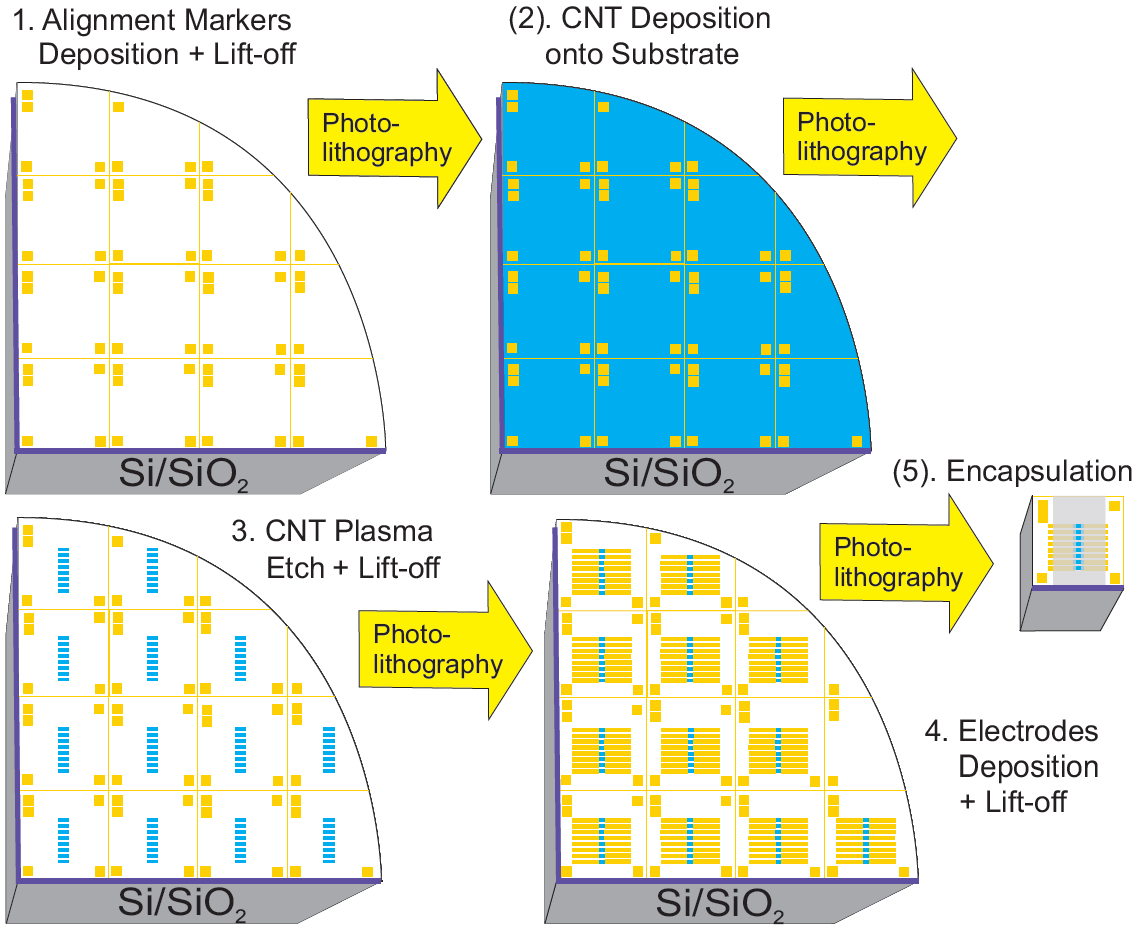
\includegraphics[width=0.9\textwidth,height=\textheight]{./figures/ch4/photolithography-cycle.png}

}

\caption{\label{fig-qw-photolithography}The photolithographic processes
used for fabrication of both carbon nanotube and graphene devices
(graphene devices were fabricated individually for every step. Step \#2
is passed over for graphene devices).}

\end{figure}

Photolithography was used to define eight channel regions on each device
and subsequently to define metal contacts for each of these channels. A
schematic demonstrating these photolithography processes on a quarter
wafer is shown in Figure~\ref{fig-qw-photolithography}. Masks for
photolithography were designed in-house using LayoutEditor CAD software
and patterned externally with a UV laser writer.

Thermal evaporation was used when depositing chromium (Cr-plated
tungsten rods, Kurt J. Lesker) and gold (Au wire, 99.99\%, Regal
Castings Ltd.), while electron beam evaporation was used when depositing
titanium (Ti pieces, 99.99\%, Kurt J. Lesker) and metal oxides
(\emph{e.g.} Al\(_2\)O\(_3\) pieces, 99.99\%, Kurt J. Lesker). Metal and
metal oxide deposition was performed using an Angstrom Engineering
Nexdep 200 Vacuum Deposition System. Deposition thickness was monitored
by a Inficon quartz piezoelectric sensor and controlled using an Inficon
Deposition Controller. Electron beam power was provided by a Telemark
TT-6 power supply. For metals, the chamber was initially evacuated to a
pressure \(5 \times 10^{-6}\) mTorr, while for metal oxides the chamber
was initially evacuated to a pressure of \(1 \times 10^{-5}\) mTorr.
After evaporation, the chamber was cooled and vented with nitrogen.

Carbon nanotube network field-effect transistors were fabricated using
4-inch \(p\)-type (B-doped) silicon wafers with either a 100 nm or 300
nm SiO\(_2\) layer (WaferPro LLC) as the substrate. Devices intended for
backgated measurements were fabricated with a 100 nm SiO\(_2\) layer.
Before photolithographic processing, the wafers were spin-coated with
AZ\(^\circledR\) 1518 photoresist, placed photoresist-side down onto a
cleanroom wipe, fixed in place using vacuum suction, then cleaved into
quarters using a diamond-tipped scribe tool. For fabrication performed
before June 2023, the protective photoresist layer was then removed by
soaking the quarter-wafers in acetone for 15 minutes, then rinsed with
isopropyl alcohol (IPA) and dried with N\(_2\) gas. However, for
complete removal of photoresist, we found it was necessary to flood
expose the wafer with the Karl Suss Aligner for 1 min and then place it
in AZ326 developer for 3 min, as discussed further in
\textbf{?@sec-photoresist-contamination}.

Graphene field-effect transistors were fabricated using 300 nm
SiO\(_2\)/p-type Si substrates covered with a monolayer of mechanically
transferred CVD graphene (Advanced Chemical Supplier). This substrate
was cleaved into equal-sized square chips before photolithography, with
side length between \(11.6-11.7\) mm, subject to variability in wafer
size. The same cleaving process outlined in
Section~\ref{sec-dep-carbon-nanotubes} was used for cleaving the chips,
but the photoresist was not rinsed off after cleaving. Devices were
exposed to a brief burst of N\(_2\) gas to remove any dust from the
cleaving process from the surface of devices. When not being used in
photolithography, graphene-based devices were stored in a vacuum
desiccator to prevent the quality of the graphene deteriorating with
exposure to air over time. The limited adhesion of graphene to the wafer
meant that photolithographic processing had to be performed particularly
carefully when fabricating graphene devices.

From Jul 2023 onwards, after each photolithography step using negative
resist, quarter wafers/chips were placed in AZ\(^\circledR\) 326 or SU8
developer for 3 min to ensure complete removal of photoresist residue.
For each step with positive resist, the same procedure was performed but
with a flood exposure with UV light for 1 min before being placed in
developer. The exception to this rule was for devices with an aluminium
oxide layer present. Tetramethylammonium hydroxide (TMAH), the active
ingredient of AZ\(^\circledR\) 326, etches through aluminium oxide and
causes electrical shorts through the dielectric layer
\autocite{Oh2011,Ali2021}. A further discussion showing the results of
this process is given in \textbf{?@sec-photoresist-contamination}.

\begin{figure}

\begin{minipage}[t]{0.25\linewidth}

{\centering 

~

}

\end{minipage}%
%
\begin{minipage}[t]{0.50\linewidth}

{\centering 

\raisebox{-\height}{

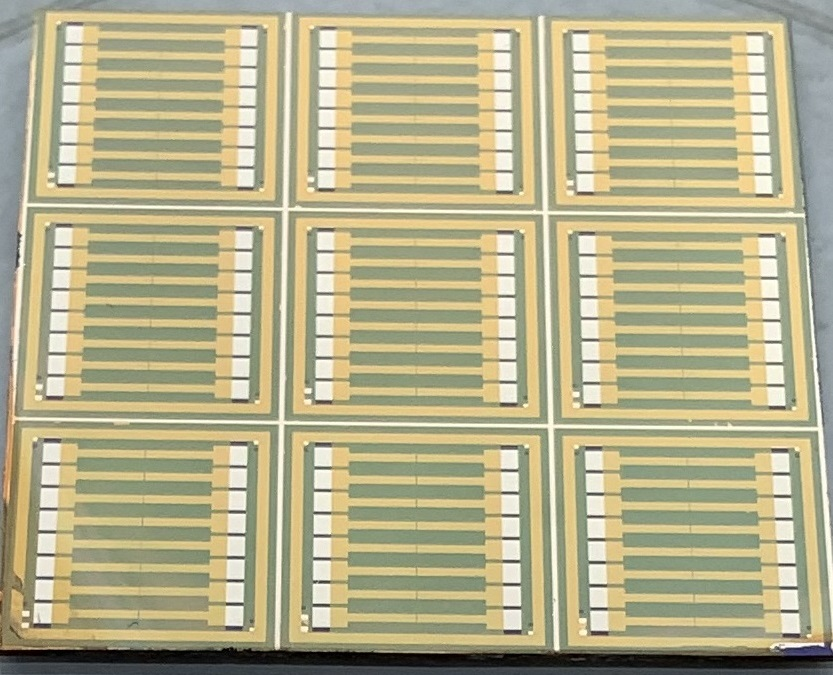
\includegraphics{./figures/ch4/IMG_0845.jpg}

}

}

\subcaption{\label{fig-qw-device-photo}}
\end{minipage}%
%
\begin{minipage}[t]{0.25\linewidth}

{\centering 

~

}

\end{minipage}%
\newline
\begin{minipage}[t]{0.47\linewidth}

{\centering 

\raisebox{-\height}{

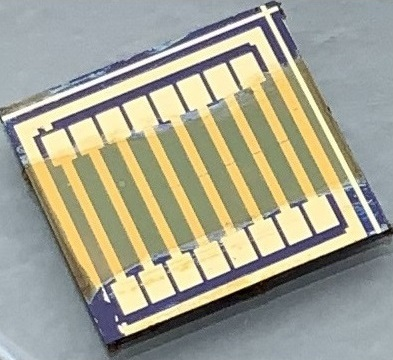
\includegraphics{./figures/ch4/IMG_0845_2.jpg}

}

}

\subcaption{\label{fig-single-device-photo}}
\end{minipage}%
%
\begin{minipage}[t]{0.05\linewidth}

{\centering 

~

}

\end{minipage}%
%
\begin{minipage}[t]{0.47\linewidth}

{\centering 

\raisebox{-\height}{

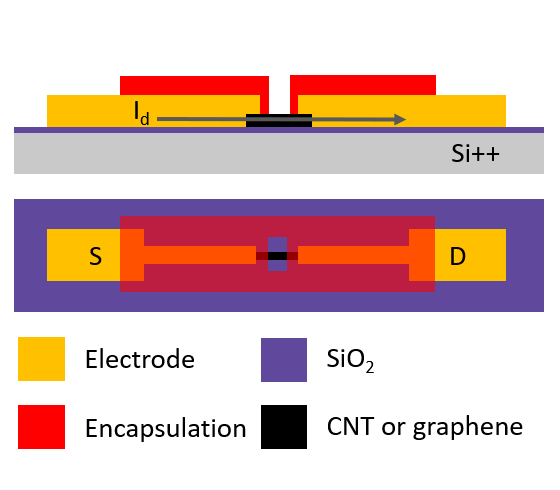
\includegraphics{./figures/ch4/fet-schematic.png}

}

}

\subcaption{\label{fig-device-schematic}}
\end{minipage}%

\caption{\label{fig-field-effect-transistor}A finished quarter-wafer
with the unusable edges cleaved off is shown in (a), while an individual
carbon nanotube field-effect transistor device is shown in (b). The
component parts of the field-effect transistor are labelled on device
cross-section and channel top view schematics in (c).}

\end{figure}

Figure~\ref{fig-qw-device-photo} shows a completed quarter-wafer of
carbon nanotube field-effect transistors, where partial (unusable)
devices at the edges of the wafer have been cleaved off so that only a
square of nine devices remains. An individual FET device after the
completed fabrication process is shown in
Figure~\ref{fig-single-device-photo}, and
Figure~\ref{fig-device-schematic} shows cross-section and top view
schematics of the completed device with the component parts labelled.

\hypertarget{sec-align}{%
\subsection{Alignment Markers}\label{sec-align}}

Metal alignment markers were deposited in order to accurately align the
device channels with device electrodes in subsequent photolithography
steps. These alignment markers were asymmetric to indicate the
orientation of the device for subsequent photolithography steps and
electrical characterisation. In later discussion, channel 1 is defined
as the channel placed closest to the large double square alignment
marker feature. For carbon nanotube quarter wafers, alignment markers
were deposited either directly before or after carbon nanotube
deposition (see Section~\ref{sec-dep-carbon-nanotubes} for discussion).
For graphene devices, alignment markers were deposited directly after
cleaving using the protective photoresist layer spincoated prior to
cleaving. AZ\(^\circledR\) 1518 was used for alignment marker
photolithography.

For carbon nanotube devices made before Jun 2022, chromium was used as
an adhesive layer for gold, while for all graphene devices and carbon
nanotube devices made after Jun 2022, titanium was used as the adhesive
layer. Metal layer thickness values quoted here are as stated on the
Inficon controller. Without first corroborating these measurements with
the Dektat profiler, these values should be treated as being strictly
nominal. For chromium/gold depositions, 10 nm of chromium was deposited
followed by a 100 nm Au layer. For titanium/gold depositions, a
\(10-20\) nm of titanium was deposited followed by a 50 nm Au layer.
Devices were then soaked in acetone for at least 2 hours for photoresist
lift-off, washed in IPA and dried with nitrogen. The use of titanium
gave rise to a cleaner lift-off and improved gold adhesion. Using a
relatively thin gold layer (50 nm nominal instead of 100 nm) proved to
still be clearly visible but to a cleaner lift-off. Profiler
measurements of combined metal layer thicknesses after lift-off are
described in Section~\ref{sec-electrodes}.

\hypertarget{sec-dep-carbon-nanotubes}{%
\subsection{Deposition of Carbon
Nanotubes}\label{sec-dep-carbon-nanotubes}}

Carbon nanotubes were deposited before the alignment markers
photolithography step on all wafers fabricated between Aug \(2021-\)Feb
2023, while devices fabricated before Aug 2021 and after Feb 2023 had
the alignment markers photolithography step performed before the
deposition of carbon nanotubes. The process order was first switched in
Aug 2021 as this order led to faster processing times. However, the
order was switched back in Feb 2023 to minimise the exposure of carbon
nanotubes to photolithographic chemical processes.

\hypertarget{solvent-based}{%
\subsubsection*{Solvent-Based}\label{solvent-based}}
\addcontentsline{toc}{subsubsection}{Solvent-Based}

The solvent-based deposition process for the carbon nanotube network in
the second fabrication protocol is as follows. 10 mg of
2-mercaptopyridine (99\%, Sigma-Aldrich) was dissolved in 1 ml ethanol
by sonication until clear. Quarter wafers were sonicated in acetone for
3 min, then exposed to O\(_2\) plasma at 100 W for at least 2 min in a
small plasma cleaner (Plasma Etch, Inc., PE-50 Compact Benchtop Plasma
Cleaning System) or reactive ion etcher (Oxford Instruments,
Plasmalab\(^\circledR\) 80 Plus) under 300 mTorr pressure. The cleaned
SiO\(_2\)/Si surface was then coated with 2-mercaptopyridine for 10
minutes, rinsed with ethanol to remove residual \(2\)-mercaptopyridine,
and then nitrogen dried.

Meanwhile, 5 \(\mu\)g of 99\% semiconducting carbon nanotube bucky paper
(NanoIntegris, IsoNanotubes S-99) was dispersed in 10 mL of anhydrous
1,2-dichlorobenzene (DCB, Sigma Aldrich) by ultrasonication until no
particles were visible to the naked eye. During this time, the
ultrasonic bath temperature was kept between \(20-30^\circ\)C or the
buckypaper would not disperse successfully. The substrates were then
placed into a dish with CNT-DCB suspension and left covered for 1 hour,
dipped into ethanol for 10 min to remove residual solvent and any
unattached carbon nanotube bundles, and then dried with nitrogen.

\hypertarget{surfactant-based}{%
\subsubsection*{Surfactant-Based}\label{surfactant-based}}
\addcontentsline{toc}{subsubsection}{Surfactant-Based}

Two different approaches were used to attach the surfactant-dispersed
carbon nanotubes (CNTs) to the substrate surface. The first approach was
a simple drop-casting method, while the second was performed in the
presence of steam (`steam-assisted'). In both approaches, the quarter
wafers were first rinsed with ultrapure deionised water (DI water),
acetone and IPA. Next, they were placed into a small plasma cleaner
(Plasma Etch, Inc, PE-50 Compact Benchtop Plasma Cleaning System) or
reactive ion etcher (Oxford Instruments, Plasmalab 80 Plus) and exposed
to O\(_2\) plasma at 100 W for at least 2 min under 300 mTorr pressure
to make the surface hydrophilic. 1 mL of poly-L-lysine (PLL) was
immediately deposited onto each quarter wafer and left for 5 minutes.
The quarter wafers were then rinsed for 30 s with DI water and dried
with N\(_2\) gas. The presence of the PLL on the plasma cleaned surface
strengthens the surface adhesion of semiconducting single carbon
nanotubes after the surfactant dispersion has been dropcast onto the
substrate.

For carbon nanotube network films deposited in surfactant without steam
present, 2 mL of IsoNanotubes-S 90\% or 99\% dispersion (NanoIntegris)
was decanted into a small bottle and sonicated for 5 s to break up
bundles of CNTs. (Note: The composition of the surfactant used in the
dispersion is proprietary to NanoIntegris.) An even spread of 400
\(\mu\)L carbon nanotube dispersion was placed in the centre of the
PLL-functionalised quarter wafer, covered with a glass dish and left for
10 minutes. The dispersion was then rinsed off with DI water and IPA,
and the quarter wafer was dried with N\(_2\) gas. Next, the quarter
wafer was annealed in a vacuum oven at 150\(^\circ\) C for 1 hour to
remove residual surfactant. This method would often lead to an
inhomogeneous spread of CNTs across the quarter wafer surface, detailed
further in section \textbf{?@sec-cnt-deposition-effects}.

\begin{figure}

\begin{minipage}[t]{0.47\linewidth}

{\centering 

\raisebox{-\height}{

\includegraphics{./figures/ch4/steaming-method-top.png}

}

}

\subcaption{\label{fig-steaming-method-top}}
\end{minipage}%
%
\begin{minipage}[t]{0.05\linewidth}

{\centering 

~

}

\end{minipage}%
%
\begin{minipage}[t]{0.47\linewidth}

{\centering 

\raisebox{-\height}{

\includegraphics{./figures/ch4/steaming-method-side.png}

}

}

\subcaption{\label{fig-steaming-method-side}}
\end{minipage}%

\caption{\label{fig-steaming-method}Top view (a) and side view (b) of
the steam-assisted method setup, with and without the glass steam cover
above the quarter wafer.}

\end{figure}

For carbon nanotube network films deposited in surfactant in the
presence of steam, 2 mL of IsoNanotubes-S 90\% or 99\% dispersion
(NanoIntegris) was decanted into a small bottle and burst-sonicated once
(on then off again) to break up bundles of carbon nanotubes. 75 mL of
95\(^\circ\) C water was then placed into a glass dish on a hotplate
held at 95\(^\circ\) C. After this, the PLL-functionalised quarter wafer
was placed in the centre of an insulating surface on the same hotplate.
The carbon nanotube dispersion was carefully spread across the surface
of the wafer without spilling any over the wafer edges. The wafer on the
insulating surface and glass dish were then left under the same glass
dish for 2 minutes to expose the wafer to steam from the glass dish. The
use of an insulating surface meant that the wafer and dispersion were
not heated from below while exposed to steam. The steam-assisted
deposition setup is shown in Figure~\ref{fig-steaming-method}.

The carbon nanotube dispersion was then rinsed off the wafer with DI
water, ethanol, acetone and IPA, and then the quarter wafer was dried
with N\(_2\) gas. As in the original method, the quarter wafer was then
annealed in a vacuum oven at 150\(^\circ\) C for 1 hour to remove
residual surfactant. This method gave an even spread of CNTs across the
quarter wafer surface, leading to a greater consistency in performance
between devices. Further details can be found in
\textbf{?@sec-cnt-deposition-effects}.

\hypertarget{channel-etching}{%
\subsection{Channel Etching}\label{channel-etching}}

Eight channel features, each 1000 \(\mu\)m in length and 100 \(\mu\)m in
width with a pitch of 1200 \(\mu\)m, were patterned using
AZ\(^\circledR\) 1518 photolithography on each carbon nanotube or
graphene-covered substrate. Unwanted nanomaterial not covered with
photoresist was then etched away with 200 W oxygen plasma at 600 mTorr
using a reactive ion etcher or RIE (Plasmalab\(^\circledR\) 80 Plus,
Oxford Instruments). The etch time was 3 minutes for carbon nanotube
quarter wafers, and 1 minute for graphene chips. The protective
photoresist was then removed by soaking in acetone for at least 5
minutes.

\begin{figure}

\begin{minipage}[t]{0.47\linewidth}

{\centering 

\raisebox{-\height}{

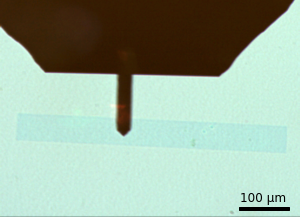
\includegraphics{./figures/ch4/channel-area.png}

}

}

\subcaption{\label{fig-graphene-channel-etch}}
\end{minipage}%
%
\begin{minipage}[t]{0.05\linewidth}

{\centering 

~

}

\end{minipage}%
%
\begin{minipage}[t]{0.47\linewidth}

{\centering 

\raisebox{-\height}{

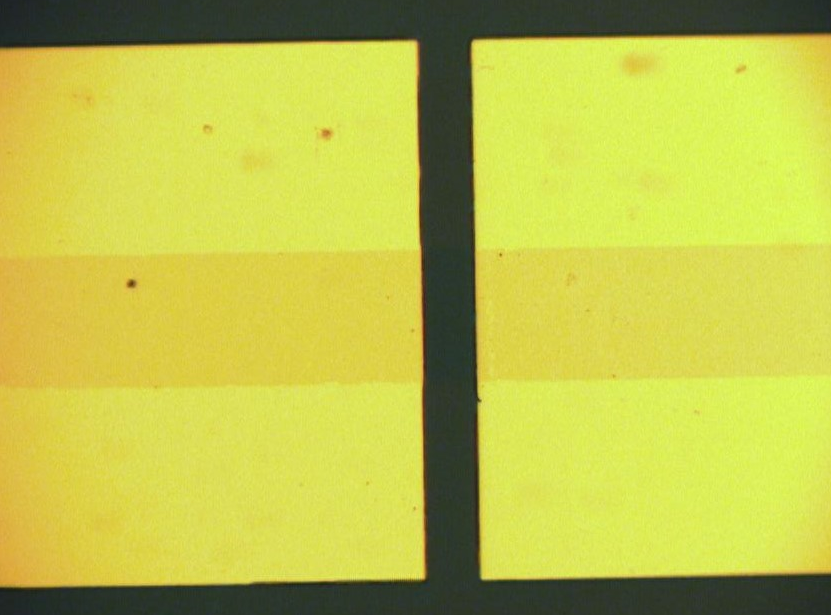
\includegraphics{./figures/ch4/graphene-channel-electrodes.png}

}

}

\subcaption{\label{fig-graphene-channel-electrodes}}
\end{minipage}%

\caption{\label{fig-microscope-graphene-channel}A graphene channel after
the plasma etch step is shown in (a), and (b) shows another graphene
channel after the metal electrode deposition and liftoff step.}

\end{figure}

\hypertarget{sec-electrodes}{%
\subsection{Source and Drain Electrodes}\label{sec-electrodes}}

\begin{figure}

\begin{minipage}[t]{0.47\linewidth}

{\centering 

\raisebox{-\height}{

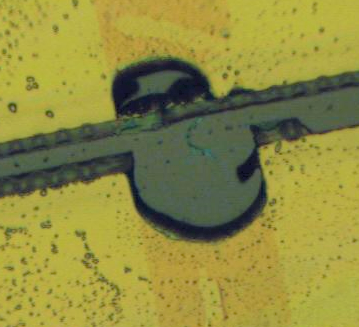
\includegraphics{./figures/ch4/apr-21-dmso-damage.png}

}

}

\subcaption{\label{fig-electrode-dmso-damage}}
\end{minipage}%
%
\begin{minipage}[t]{0.05\linewidth}

{\centering 

~

}

\end{minipage}%
%
\begin{minipage}[t]{0.47\linewidth}

{\centering 

\raisebox{-\height}{

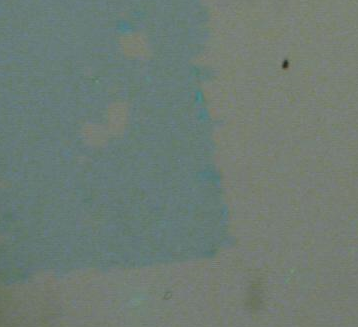
\includegraphics{./figures/ch4/may-21-dmso-damage.png}

}

}

\subcaption{\label{fig-graphene-dmso-damage}}
\end{minipage}%

\caption{\label{fig-dmso-damage}Damage to the gold electrode in the
graphene channel region after dimethyl sulfoxide lift-off is shown in
(a), while (b) shows damage to a graphene film (blue-green region) after
dimethyl sulfoxide lift-off.}

\end{figure}

\begin{figure}

\begin{minipage}[t]{0.47\linewidth}

{\centering 

\raisebox{-\height}{

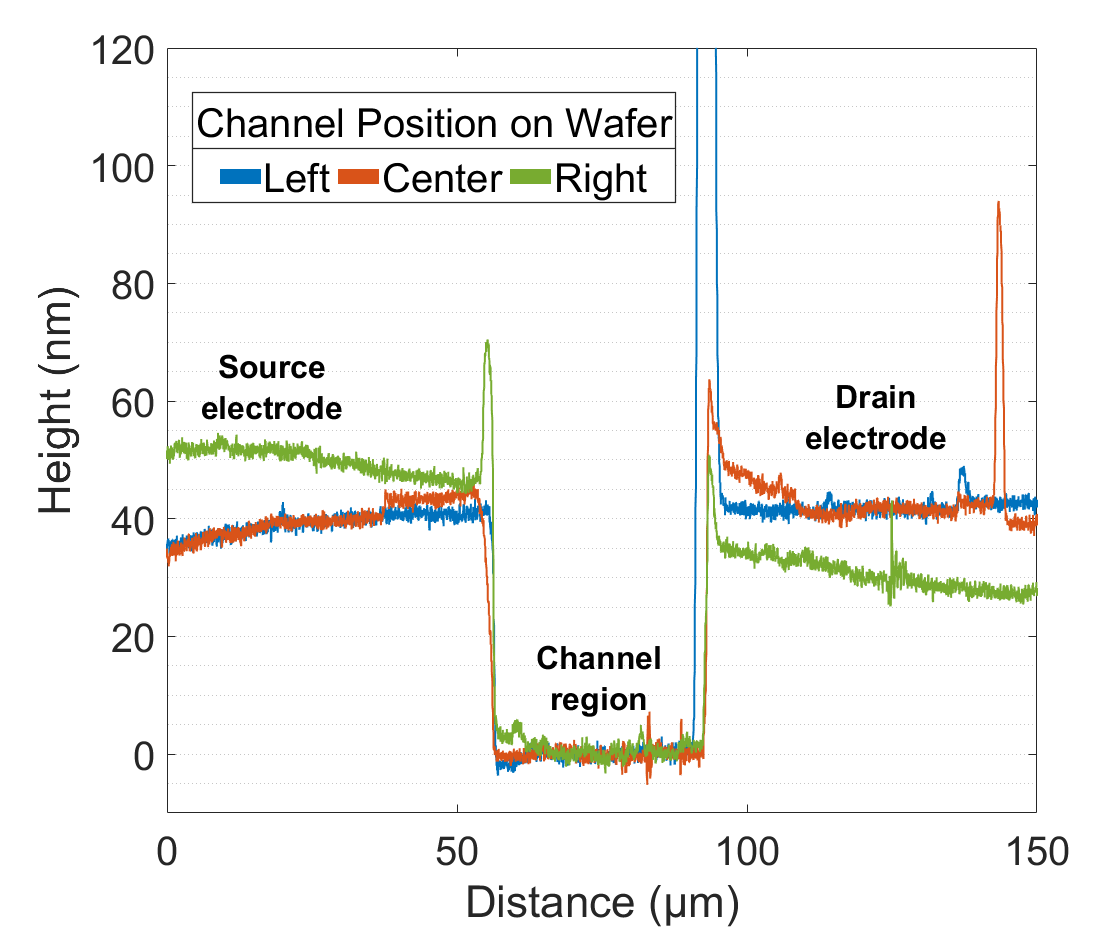
\includegraphics{./figures/ch4/dektat_cr_electrodes.png}

}

}

\subcaption{\label{fig-dektat-cr}}
\end{minipage}%
%
\begin{minipage}[t]{0.05\linewidth}

{\centering 

~

}

\end{minipage}%
%
\begin{minipage}[t]{0.47\linewidth}

{\centering 

\raisebox{-\height}{

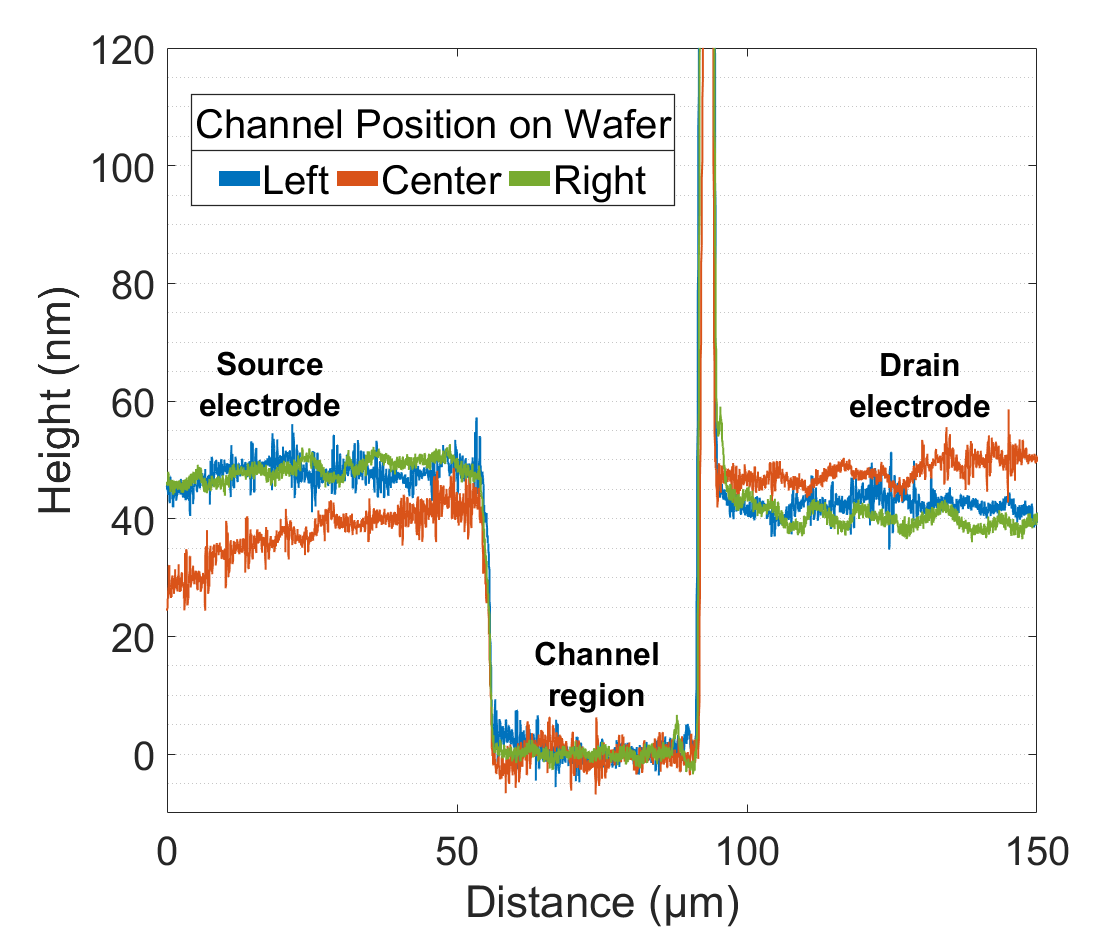
\includegraphics{./figures/ch4/dektat_ti_electrodes.png}

}

}

\subcaption{\label{fig-dektat-ti}}
\end{minipage}%
\newline
\begin{minipage}[t]{0.47\linewidth}

{\centering 

\raisebox{-\height}{

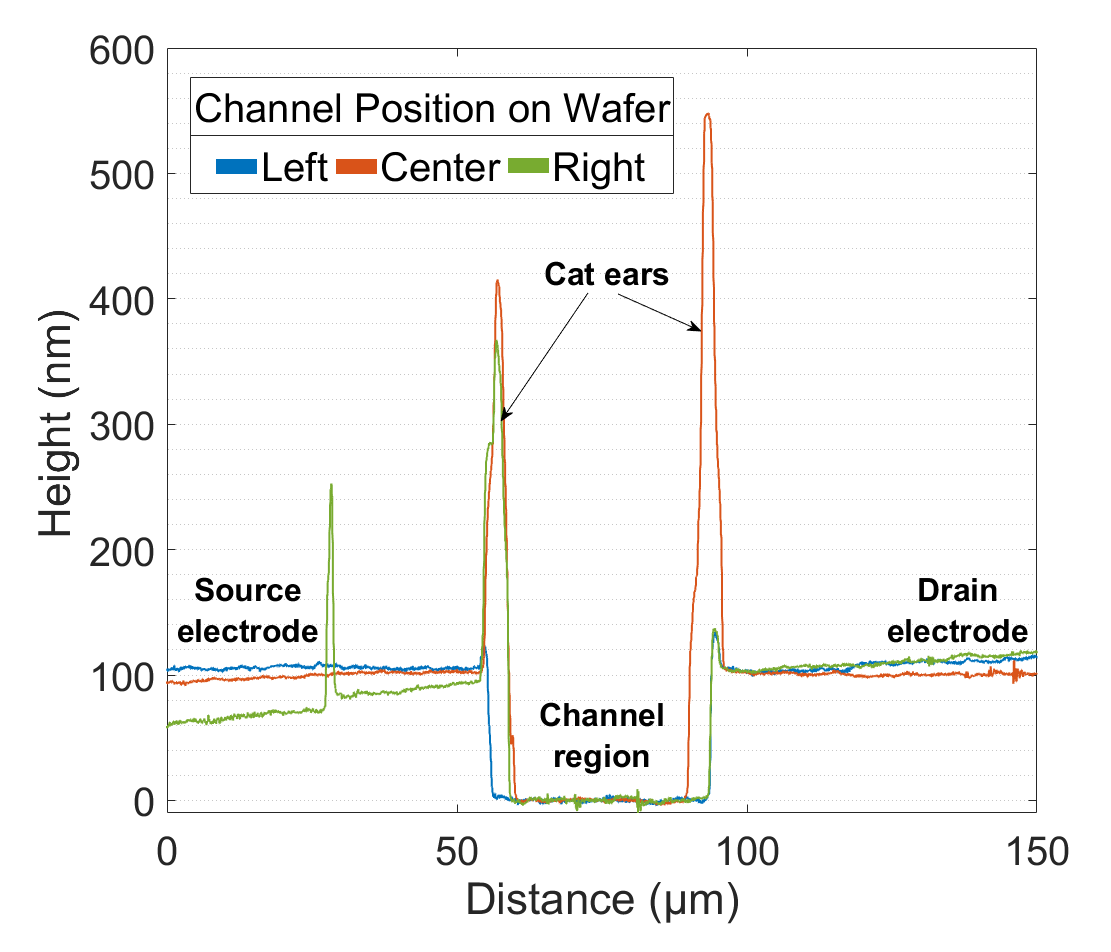
\includegraphics{./figures/ch4/dektat_1518_electrode_profile.png}

}

}

\subcaption{\label{fig-dektat-AZ1518-electrode}}
\end{minipage}%
%
\begin{minipage}[t]{0.05\linewidth}

{\centering 

~

}

\end{minipage}%
%
\begin{minipage}[t]{0.47\linewidth}

{\centering 

\raisebox{-\height}{

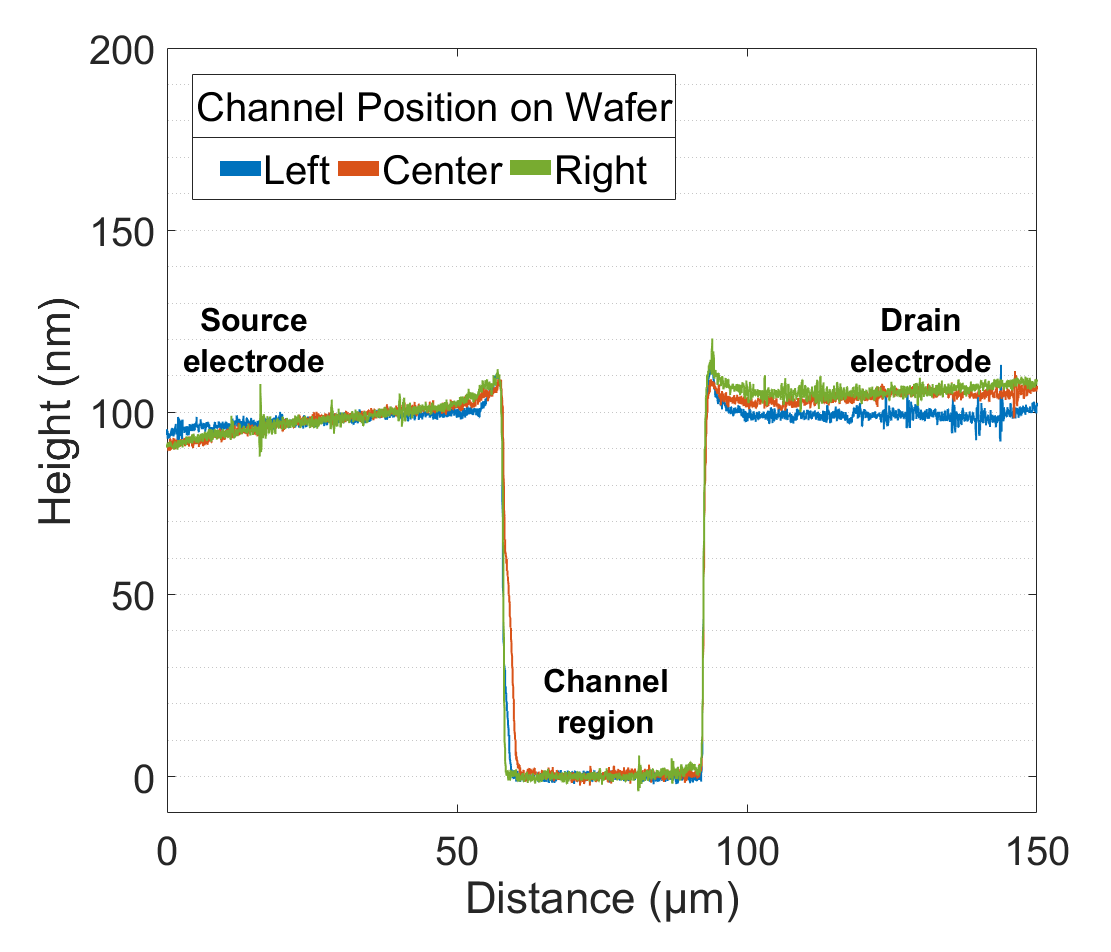
\includegraphics{./figures/ch4/dektat_nlof_electrode_profile_2.png}

}

}

\subcaption{\label{fig-dektat-nLOF-electrode}}
\end{minipage}%

\caption{\label{fig-electrodes-dektat}The Dektat height profile
measurements for source and drain electrodes taken at different
locations on four different quarter wafers are shown here. Chromium was
used as an adhesion layer for the wafer in (a), while titanium was used
as the adhesion layer in (b) and (c). AZ\(^\circledR\) 1518
photolithography was used for patterning before metal deposition on both
quarter wafers, which led to the formation of edge features or ``cat
ears'', with (c) illustrating the full height of these features. In
comparison, (d) shows the profile of electrodes from a quarter wafer
patterned with AZ\(^\circledR\) nLOF2020, where edge features are
greatly reduced.}

\end{figure}

The source and drain electrodes for each channel were patterned using
photolithography with either AZ\(^\circledR\) 1518 photoresist (pre-Mar
2023) or AZ\(^\circledR\) nLOF 2020 photoresist (post-Mar 2023). Before
metal deposition, the developed photoresist pattern was exposed to
O\(_2\) plasma at 50 W for up to 5 s or at 20 W for \(20-25\) s in a
PE-50 plasma cleaner (Plasma Etch, Inc.) to remove residual photoresist
on the developed regions and ensure a clean lift-off. After metal
deposition, wafers/devices were soaked in acetone for at least 2 hours
for photoresist lift-off, washed in IPA and dried with nitrogen.

As with the alignment markers deposition (see Section~\ref{sec-align}),
before Jun 2022 chromium was used for the gold adhesion layer, and after
Jun 2022 titanium was used. Adhesion layers are required to stick metals
such as gold and platinum to silicon dioxide \autocite{Guarnieri2014}. A
20 nm nominal titanium layer instead of 10 nm nominal was found to give
better electrode adhesion, and devices after Feb 2023 were made using
this thicker adhesion layer. Good electronic contact could be made with
electrodes with a nominal gold layer thickness of \(60-100\) nm, and a
Au layer nominally 100 nm thick was most commonly used.

Dimethyl sulfoxide (DMSO) was sometimes used in electrodes lift-off
instead of acetone between Jul 2021 and Feb 2023 because of its
effectiveness as a photoresist stripping agent. However, it was
abandoned due to some indications it was unsuitable for the devices
being fabricated, as shown in Figure~\ref{fig-dmso-damage} and also as
detailed in \textbf{?@sec-cnt-deposition-effects}. It is possible that
heat from the electrodes deposition sometimes crosslinked residual
photoresist on the nanomaterial, and then during lift-off was removed
together with any attached nanomaterial by the DMSO. However, it is also
possible that prolonged exposure to DMSO alone was sufficient to detach
nanomaterial from the substrate. Therefore, acetone was the preferred
agent for lift-off despite being a less efficient stripping agent than
DMSO.

Example height profiles of quarter wafer channels taken using a Veeco
Dektat 150 profiler are shown in Figure~\ref{fig-electrodes-dektat}.
AZ\(^\circledR\) 1518 photoresist was used in Figure~\ref{fig-dektat-cr}
and Figure~\ref{fig-dektat-ti} for photolithographic patterning. A 10 nm
adhesion layer and 100 nm Au layer were used for each quarter wafers to
ensure a consistent comparison. From these figures, we find an measured
Cr/Au electrode height of \(42\pm1\) nm and an measured Ti/Au electrode
height of \(48\pm2\) nm, slightly less than half the respective heights
stated on the Inficon Deposition Controller.

Although using AZ\(^\circledR\) nLOF 2020 photolithography involves more
processing steps, it gave rise to more cleanly-defined electrodes with a
more consistent height profile. Often electrode deposition using
AZ\(^\circledR\) 1518 photoresist would lead to sharp vertical spikes
along the edge of the electrode, as seen in
Figure~\ref{fig-dektat-AZ1518-electrode}. These edge spikes or ``cat
ears'' can partially or fully protrude through thin encapsulation
materials such as SU8 and Al\(_2\)O\(_3\), leading to significant
leakage currents from the electrodes into the FET top gate. This effect
is due to the profile of positive resists being suboptimal for lift-off
processes, as discussed in Section~\ref{sec-photolithography}.

The height profile corresponding to a wafer with electrodes fabricated
using AZ\(^\circledR\) nLOF 2020 is shown in
Figure~\ref{fig-dektat-nLOF-electrode}. A 20 nm titanium adhesion layer
and 100 nm Au layer were used for both
Figure~\ref{fig-dektat-AZ1518-electrode} and
Figure~\ref{fig-dektat-nLOF-electrode} to ensure a consistent
comparison, resulting in a measured electrode height of \(103\pm2\) nm
for both wafers. By comparing these figures, we see AZ\(^\circledR\)
nLOF 2020 photoresist has a more consistent electrode height profile
across the wafer surface than the wafer which used AZ\(^\circledR\) 1518
resist. The measured edge features for the AZ\(^\circledR\) 1518 resist
electrodes vary in size from 20 nm to 450 nm above the bulk electrode
surface, whereas the edge features for the AZ\(^\circledR\) nLOF 2020
resist do not exceed 14 nm in height.

\hypertarget{sec-encapsulation}{%
\subsection{Encapsulation}\label{sec-encapsulation}}

Several different approaches were used for the encapsulation, or contact
protection, of devices. The encapsulation of graphene and
carbon-nanotube transistors for biosensing is essential to improve
transistor characteristics, passivate the electrodes and ensure only the
nanomaterial region is active during biosensing, as discussed in
\textbf{?@sec-biosensor-methods}.

Before encapsulation photolithography the carbon-nanotube network
quarter wafers were cleaved into individual 11 mm \(\times\) 11 mm
chips, using the cleaving process outlined in
Section~\ref{sec-dep-carbon-nanotubes}. Cleaving the devices at this
step simplified mask alignment and ensured consistent thickness across
photoresist encapsulated devices.

Two different photolithography masks were used for encapsulation
photolithography in this work, with different exposed areas of active
nanomaterial. The first mask was used for devices made before Jan 2023,
and was designed to leave a region of 500 \(\mu\)m \(\times\) 10
\(\mu\)m unencapsulated for each channel. The second mask was used
exclusively after Jan 2023, and was designed to leave a region of 200
\(\mu\)m \(\times\) 20 \(\mu\)m unencapsulated for each channel. This
change was made to double the area of carbon nanotubes exposed to
electrolyte while halving the area of SiO\(_2\) dielectric exposed to
electrolyte during aqueous sensing.

\begin{figure}

\begin{minipage}[t]{0.47\linewidth}

{\centering 

\raisebox{-\height}{

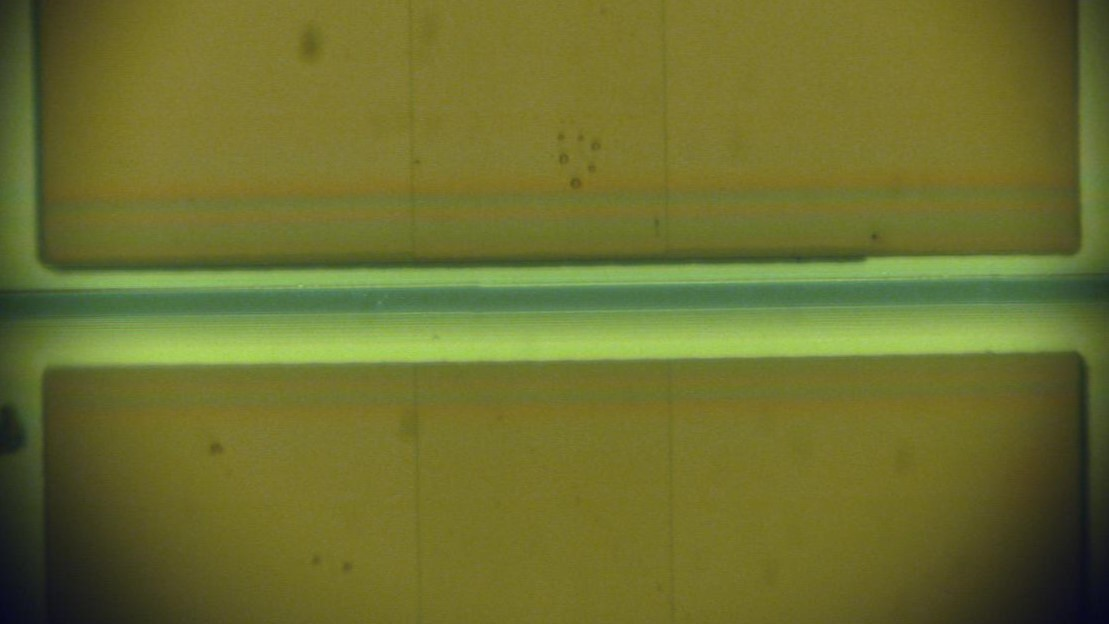
\includegraphics{./figures/ch4/encapsulation_old.png}

}

}

\subcaption{\label{fig-encapsulation-old}Encapsulation with
AZ\(^\circledR\) 1518 using pre-2023 mask}
\end{minipage}%
%
\begin{minipage}[t]{0.05\linewidth}

{\centering 

~

}

\end{minipage}%
%
\begin{minipage}[t]{0.47\linewidth}

{\centering 

\raisebox{-\height}{

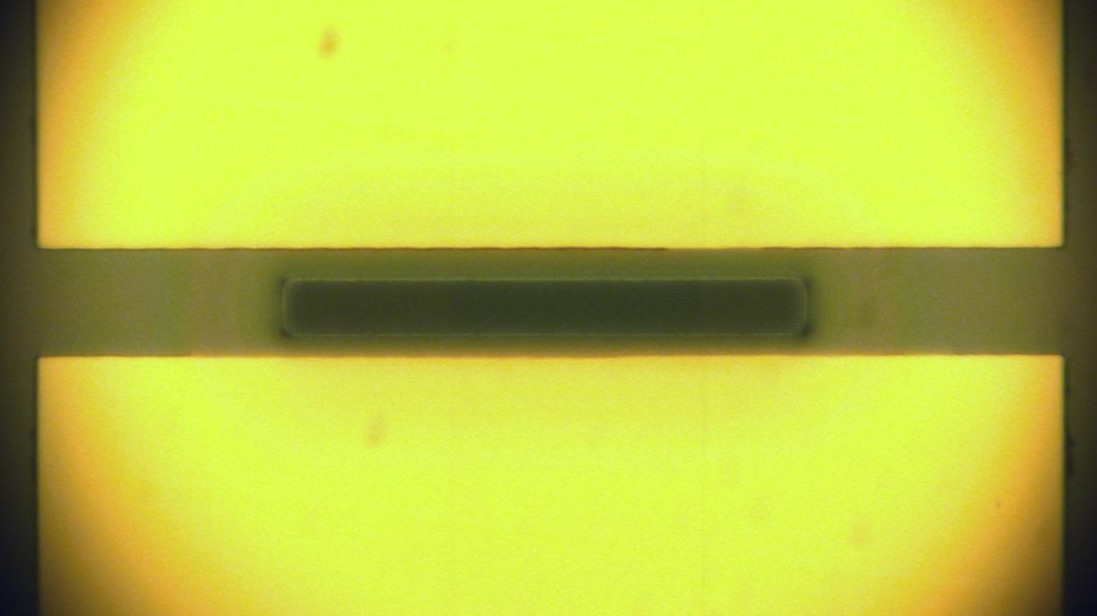
\includegraphics{./figures/ch4/encapsulation_new.png}

}

}

\subcaption{\label{fig-encapsulation-new}Encapsulation with
AZ\(^\circledR\) 1518 using 2023 mask}
\end{minipage}%

\caption{\label{fig-microscope-encapsulation}Microscope images of carbon
nanotube devices after encapsulation photolithography with hardbaked
AZ\(^\circledR\) 1518.}

\end{figure}

A side-by-side microscope comparison of hardbaked AZ\(^\circledR\) 1518
processed with each mask is given in
Figure~\ref{fig-microscope-encapsulation}, while a Dektat profile
comparison corresponding to Figure~\ref{fig-microscope-encapsulation} is
shown in \textbf{?@fig-old-new-mask}. The profiles corresponding to the
mask used after Jan 2023 clearly exhibit greater device-to-device
consistency, partly due to the mask requiring a greater level of
accuracy when aligning the encapsulation pattern with the electrode
channel. The larger feature size also means development time has less of
an impact on the quality of the encapsulation opening.

\hypertarget{photoresist-encapsulation}{%
\subsubsection*{Photoresist
encapsulation}\label{photoresist-encapsulation}}
\addcontentsline{toc}{subsubsection}{Photoresist encapsulation}

\begin{figure}

\begin{minipage}[t]{0.47\linewidth}

{\centering 

\raisebox{-\height}{

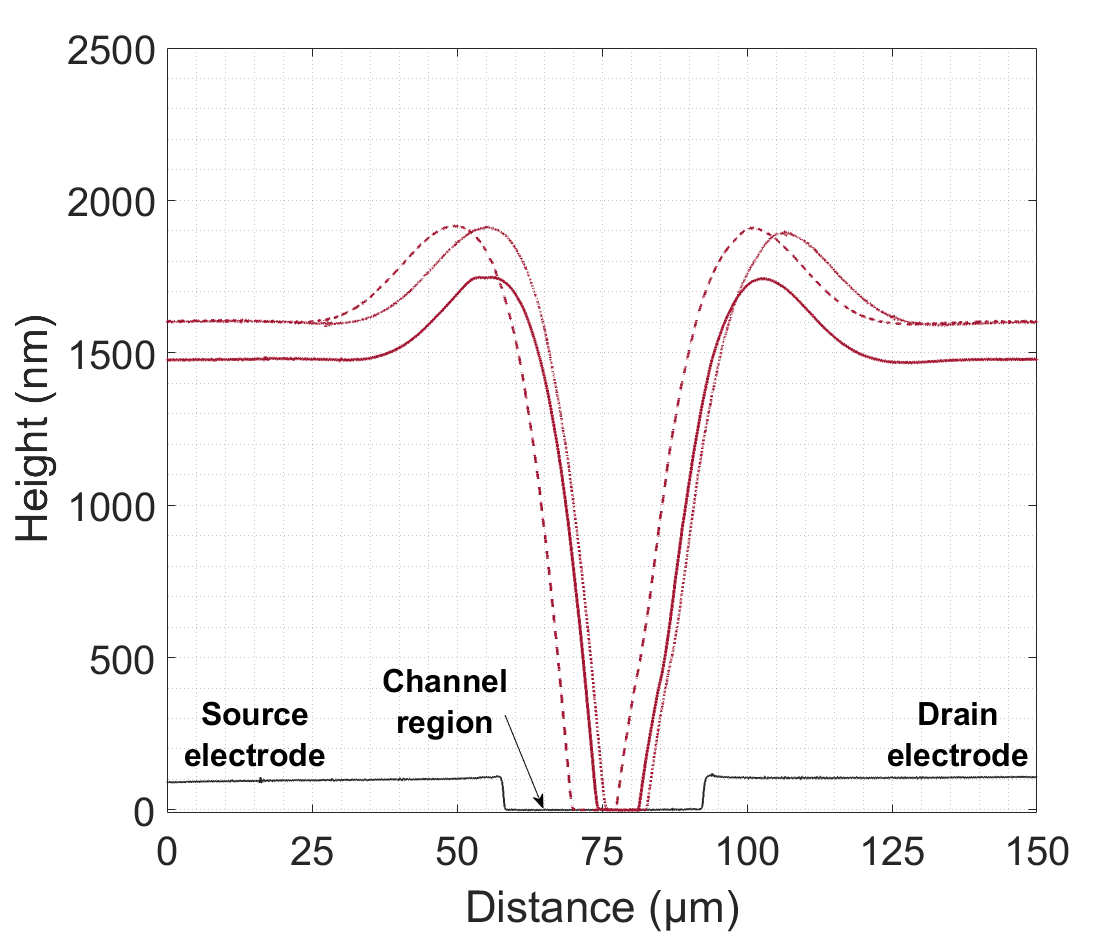
\includegraphics{./figures/ch4/dektat_AZ1518_oldmask.png}

}

}

\subcaption{\label{fig-AZ1518-old}}
\end{minipage}%
%
\begin{minipage}[t]{0.05\linewidth}

{\centering 

~

}

\end{minipage}%
%
\begin{minipage}[t]{0.47\linewidth}

{\centering 

\raisebox{-\height}{

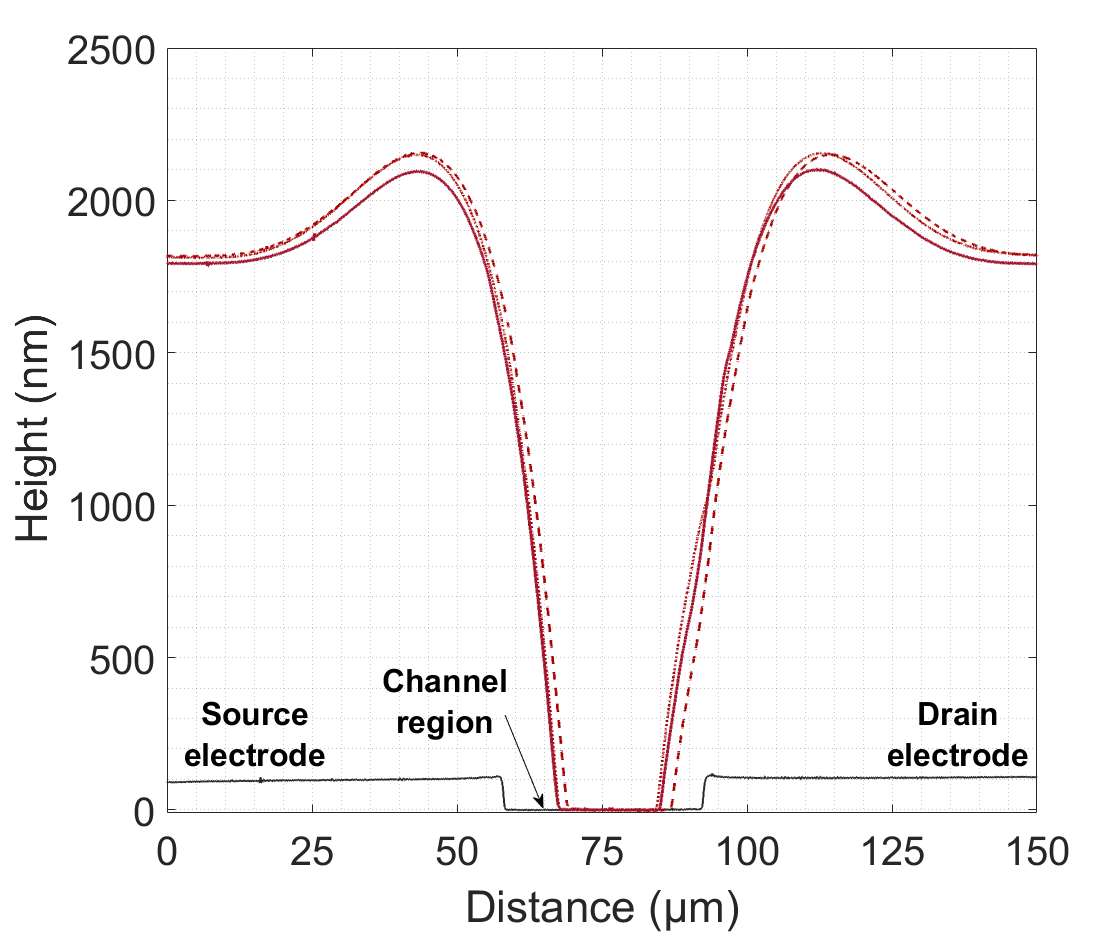
\includegraphics{./figures/ch4/dektat_AZ1518_newmask.png}

}

}

\subcaption{\label{fig-AZ1518-new}}
\end{minipage}%
\newline
\begin{minipage}[t]{0.47\linewidth}

{\centering 

\raisebox{-\height}{

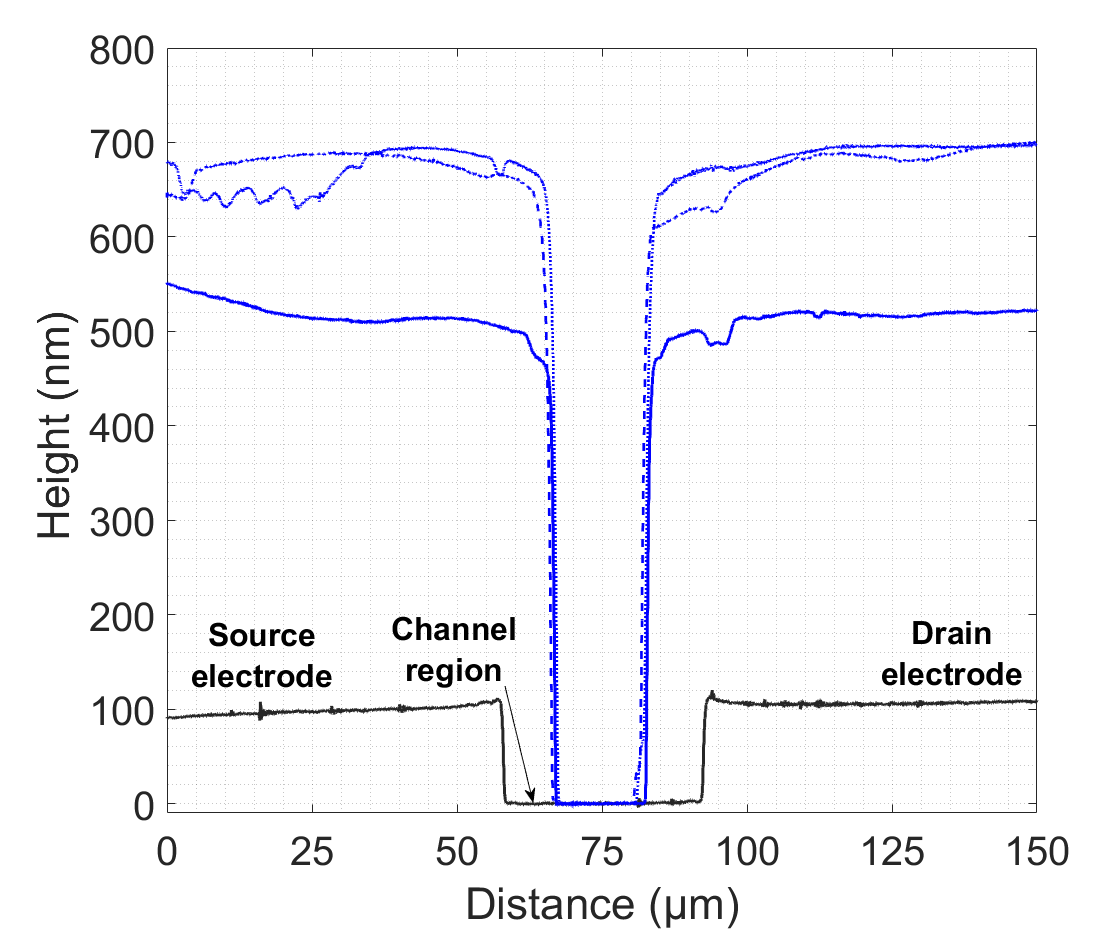
\includegraphics{./figures/ch4/dektat_SU8_newmask.png}

}

}

\subcaption{\label{fig-SU8-new}}
\end{minipage}%
%
\begin{minipage}[t]{0.05\linewidth}

{\centering 

~

}

\end{minipage}%
%
\begin{minipage}[t]{0.47\linewidth}

{\centering 

\raisebox{-\height}{

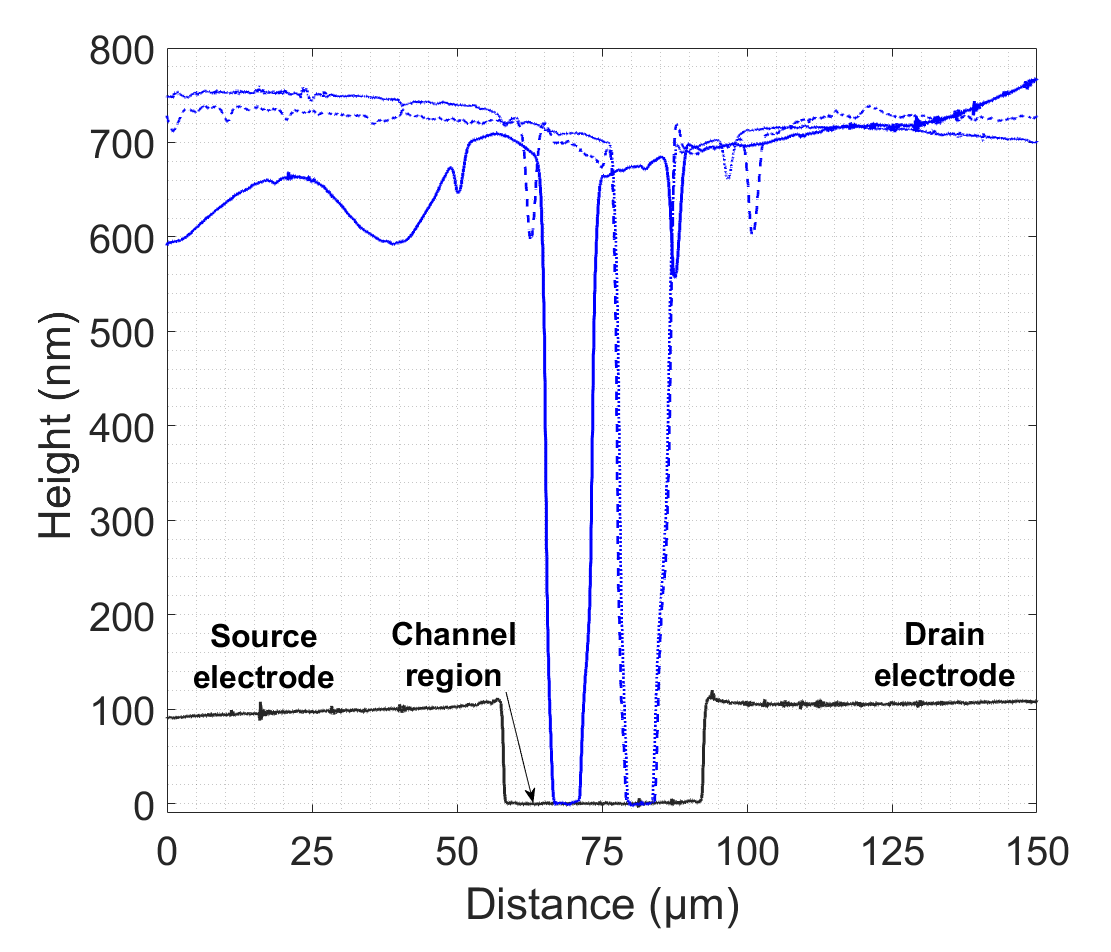
\includegraphics{./figures/ch4/dektat_SU8_oldmask.png}

}

}

\subcaption{\label{fig-SU8-old}}
\end{minipage}%

\caption{\label{fig-dektat-encapsulation}Dektat of carbon nanotube
devices after encapsulation photolithography using hardbaked
AZ\(^\circledR\) 1518 and SU-8 2150, taken from various devices. (a) and
(c) show photolithography performed with the old, pre-2023 mask, using
AZ\(^\circledR\) 1518 and SU-8 2150 respectively. (b) and (d) show
photolithography performed with the new mask from 2023 onwards, using
AZ\(^\circledR\) 1518 and SU-8 2150 respectively.}

\end{figure}

Two types of photoresist were initially trialled for encapsulation of
carbon nanotube network devices, AZ\(^\circledR\) 1518 and SU8-2150.
Both AZ\(^\circledR\) 1518
\autocite{Thanihaichelvan2018,Thanihaichelvan2019,Shkodra2021} and SU-8
have been previously used for device encapsulation, with SU-8 noted for
being particularly stable and biocompatible
\autocite{Lee2006,Chen2021,Albarghouthi2022}.

Once developed, the photoresist pattern was exposed to O\(_2\) plasma at
50 W for up to 5 s or at 20 W for \(20-25\) s to remove excess
photoresist from the encapsulation opening. Devices were then hardbaked
at 200\(^\circ\)C for 1 hour to fully crosslink the encapsulation layer.
This crosslinking ensured subsequent device exposure to solvent did not
remove the photoresist encapsulation.

The exposed region clear of AZ \(^\circledR\) 1518 resist was
\(6.8 \pm 0.3\) \(\mu\)m in width when using the old, pre-2023 mask,
while the exposed region was \(16.6 \pm 0.4\) \(\mu\)m when using
AZ\(^\circledR\) 1518 with the new mask from 2023, as seen in
Figure~\ref{fig-AZ1518-old} and Figure~\ref{fig-AZ1518-new}. However,
the exposed region was reduced for the SU-8 encapsulation relative to
the AZ\(^\circledR\) 1518, with an width of only 3.6 \(\pm\) 0.5
\(\mu\)m for the pre-2023 mask, as seen in Figure~\ref{fig-SU8-old}.
Photoresist development using SU-8 was significantly more time-sensitive
than for the AZ\(^\circledR\) 1518. This meant when the development time
was increased to create a wider encapsulation opening, it was difficult
to avoid removing large areas of photoresist across the entire surface
of the encapsulation. This meant using the new mask from 2023 was
especially important for maximising the exposed channel region of SU-8
devices. From Figure~\ref{fig-SU8-new}, we see the new mask from 2023
with the SU-8 resist gave a significantly improved width of 13.8 \(\pm\)
1.0 \(\mu\)m for the exposed region.

A relatively thin SU-8 encapsulation layer could be deposited when
compared to the AZ\(^\circledR\) 1518 encapsulation profile. From
Figure~\ref{fig-dektat-encapsulation}, we see that the AZ\(^\circledR\)
1518 encapsulation layer had a average height of 1.7 \(\pm\) 0.2
\(\mu\)m, while the SU-8 encapsulation layer had a average height of 680
\(\pm\) 20 nm. The SU-8 also had much less significant edge features
than the AZ\(^\circledR\) 1518, regardless of the profiles of the source
and drain electrodes.

As noted previously, for both resists the overall profile was more
consistent for the new, 2023 mask from device to device than for the old
pre-2023 mask.

AZ\(^\circledR\) 1518 encapsulation was used for all graphene devices
fabricated.

\hypertarget{dielectric-encapsulation}{%
\subsubsection*{Dielectric
encapsulation}\label{dielectric-encapsulation}}
\addcontentsline{toc}{subsubsection}{Dielectric encapsulation}

Another approach taken was encapsulation of electrode channels with a
dielectric metal oxide/ceramic layer. A electron beam deposition process
was used to deposit a \(100-150\) nm nominal metal oxide layer on
devices patterned with the 2023 mask using AZ\(^\circledR\) nLOF 2020
photoresist. As in Section~\ref{sec-electrodes}, the developed
photoresist pattern was exposed to O\(_2\) plasma at 50 W for up to 5 s
or at 20 W for \(20-25\) s in a PE-50 plasma cleaner (Plasma Etch, Inc.)
before ceramic deposition. Before May 2023, devices were left in
TechniStrip\(^\circledR\) MLO 07 (MicroChemicals) for \(5-10\) min for
lift-off. However, due to concerns over the impact of the constituent
chemical DMSO on the nanomaterial region (see
Figure~\ref{fig-dmso-damage}), the lift-off process was altered from May
2023 onwards. After May 2023, devices were soaked in acetone for at
least 4 hours and sonicated in clean acetone for \(30-60\) s to lift-off
the photoresist, then washed in IPA and dried with nitrogen.

\begin{figure}

\begin{minipage}[t]{0.50\linewidth}

{\centering 

\raisebox{-\height}{

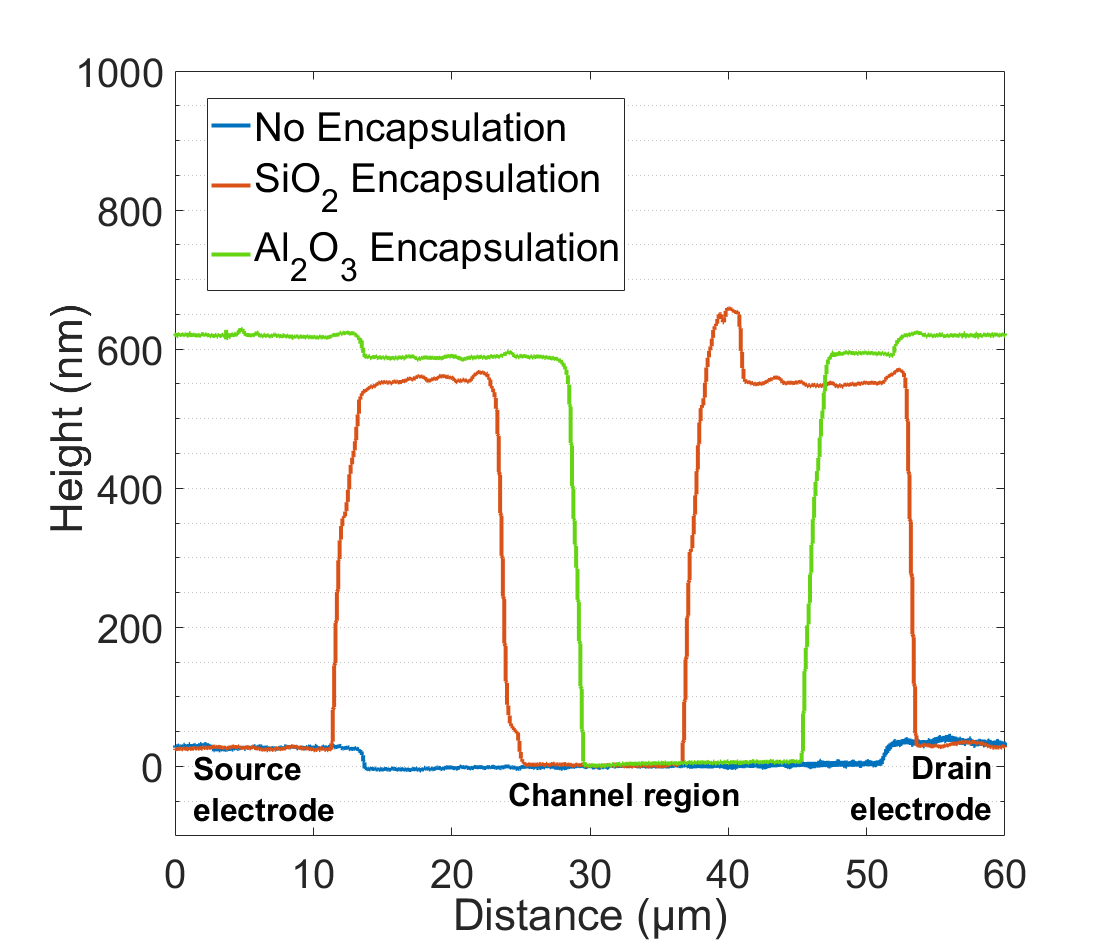
\includegraphics{./figures/ch4/Dielectric_Profile_comparison.png}

}

}

\subcaption{\label{fig-dielectric-comparison}}
\end{minipage}%
%
\begin{minipage}[t]{0.05\linewidth}

{\centering 

~

}

\end{minipage}%
%
\begin{minipage}[t]{0.45\linewidth}

{\centering 

\raisebox{-\height}{

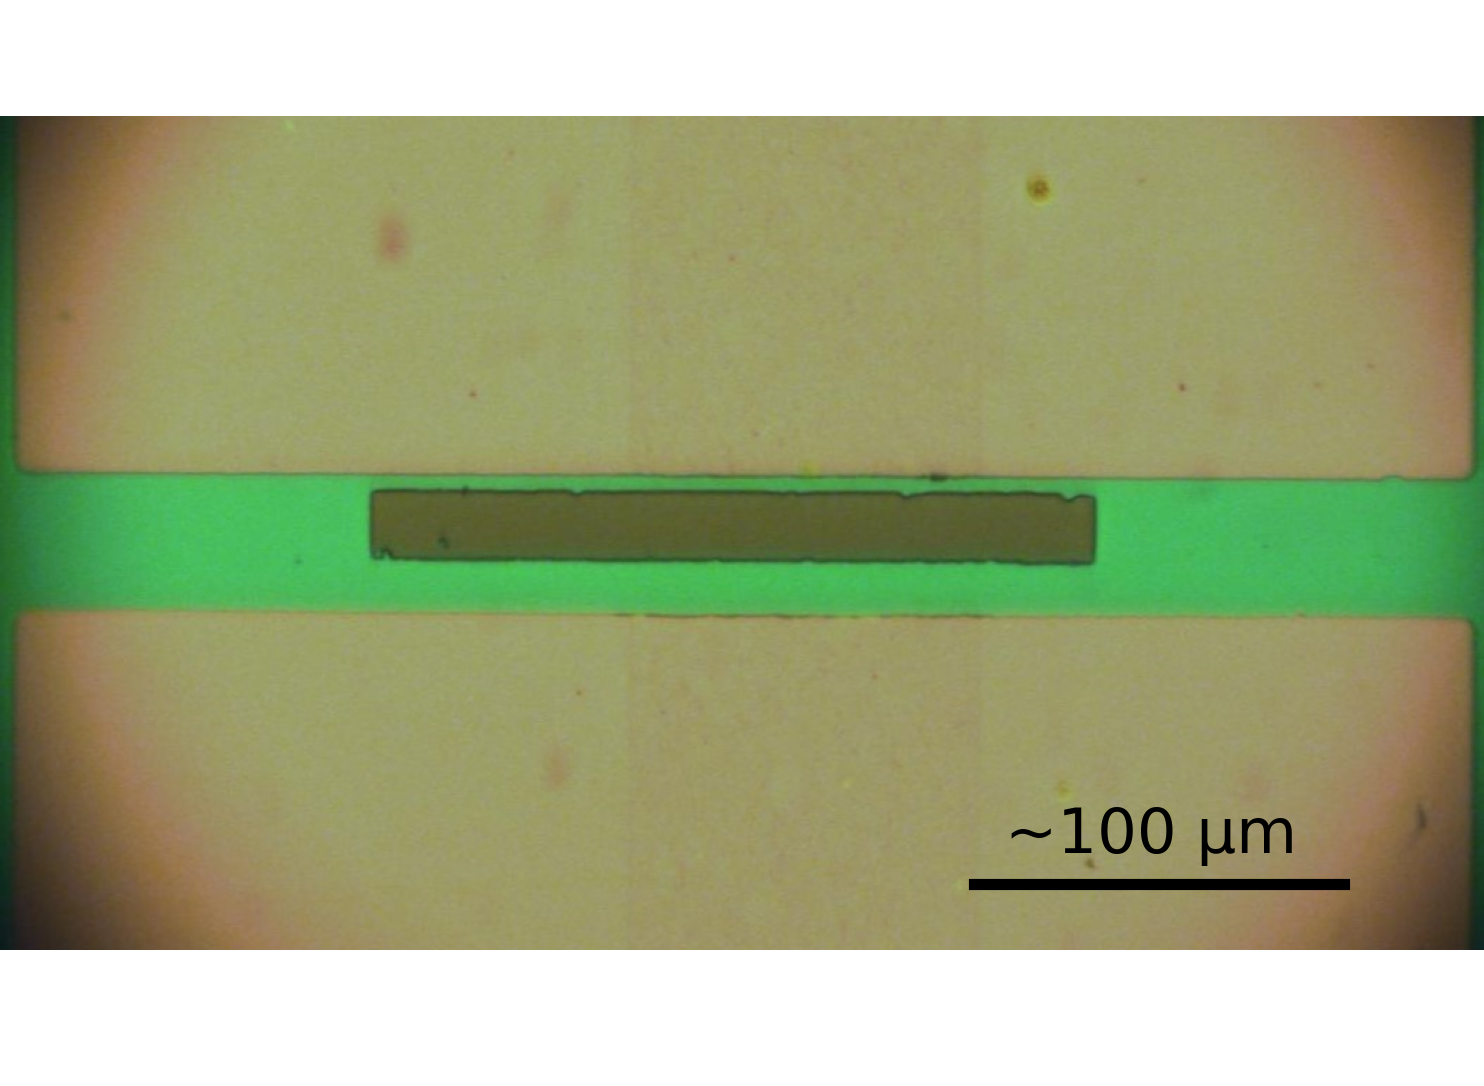
\includegraphics{./figures/ch4/al2o3_encapsulation.png}

}

}

\subcaption{\label{fig-al2o3-encapsulation}}
\end{minipage}%

\caption{\label{fig-dektat-dielectric-layer}A profile comparison of
dielectric materials used for encapsulation is shown in (a), alongside a
microscope image of a device encapsulated with aluminium oxide in (b).
Note that the layer thicknesses in (a) were from initial tests of the
process and are used for illustrative purposes.}

\end{figure}

The initial attempt at fabricating a dielectric encapsulation layer used
silicon dioxide as the dielectric. However, silicon dioxide adheres
poorly to gold without an metallic adhesive layer present, as shown in
Figure~\ref{fig-dielectric-comparison}. Aluminium oxide was chosen as an
alternative as it sticks well to bulk electrode materials, is heat and
chemical resistant, has a relatively high dielectric constant and is
bio-compatible \autocite{Guarnieri2014,Albarghouthi2022,Kolodzey2000}.
Figure~\ref{fig-dektat-dielectric-layer} shows the aluminium oxide
successfully adhered to the electrodes and had a clean profile
comparable to that of the SU-8 encapsulation layer after lift-off.

Unfortunately, when aluminium oxide layers which were thicker than
\(\sim\) 100 nm were deposited, there was found to be a significant drop
in current relative to the unencapsulated device. This drop was
signficant enough to make devices unsuitable for sensing. Meanwhile,
devices with encapsulation \(\sim\) 100 nm thick had significant gate
current leakage through the encapsulation layer when liquid-gated. This
leakage was present even when AZ\(^\circledR\) nLOF 2020 was used for
electrode patterning to avoid edge spikes (as discussed in
Section~\ref{sec-electrodes}). Furthermore, aluminium oxide should not
be subsequently exposed to its etchant TMAH, meaning it was difficult to
completely remove residual photoresist from device channels after
encapsulation. Possible future approaches to ceramic encapsulation are
discussed in \textbf{?@sec-future-work}.

\hypertarget{sec-afm-characterisation}{%
\section{Characterisation via Atomic Force
Microscopy}\label{sec-afm-characterisation}}

Atomic force microscopy in this thesis was taken using a Nanosurf
NaioAFM in dynamic force mode (also known as tapping mode, oscillating
mode, acoustic AC mode or intermittent-contact mode). An ACLA probe
(AppNano) was used with a tip diameter of 12 nm, height of \(14-16\)
\(\mu\)m and a nominal cantilever spring constant of 58 N/m. All atomic
force microscopy was performed with the Nanosurf NaioAFM on a stablising
table under a Faraday cage to minimise mechanical and electromagnetic
interference. A 256 \(\times\) 256 pixel resolution was typically used.
Imaging was performed in air at room temperature.

Atomic force microscope (AFM) images could not be taken from the small
exposed channel region on the encapsulated devices, so were instead
taken on a representative carbon nanotube or graphene film sample
fabricated on the same wafer as the device being tested. Moisture
adversely affected the AFM imaging process. Therefore, films
functionalised with biological materials were washed with DI water and
gently dried with N\(_2\) before atomic force microscope images were
taken.

The open source data analysis software Gwyddion (version 2.59) was used
to analyse AFM images. This included levelling the background with the
polynomial background removal function, removing scarring and zeroing
the z-scale.

\hypertarget{sec-fluorescence-characterisation}{%
\section{Characterisation via Fluorescence
Microscopy}\label{sec-fluorescence-characterisation}}

Fluorescence microscopy was performed using an Olympus BX63 fluorescence
microscope controlled using cellSens imaging software. Microscope
objectives used were all Olympus UPLSAPO/UPlanSApo, apochromat
objectives which compensate for spherical and chromatic aberrations.
Objectives had infinite aperture and a field number of 26.5. Filter
cubes used included the Olympus FITC filter (excitation wavelength
range: \(467-498\) nm, emission wavelength range: \(513-556\) nm), Texas
Red (excitation wavelength range: \(542-582\) nm, emission wavelength
range: \(604-644\) nm) and GFP (excitation wavelength range: \(604-644\)
nm, emission wavelength range: \(502-538\) nm). The ISO was kept at the
lowest available setting, ISO200. All microscopy was performed in
darkness with the screen turned away from the microscope. To ensure
photobleaching did not adversely affect imaging, images were taken soon
after initial exposure to fluorescence and taking repeated photos of the
same region was avoided. Various useful and thorough introductions to
fluorescence microscopy can be found online \autocite{Nikon,Zeiss}.

\hypertarget{sec-electrical-characterisation}{%
\section{Electrical
Characterisation}\label{sec-electrical-characterisation}}

\begin{figure}

{\centering 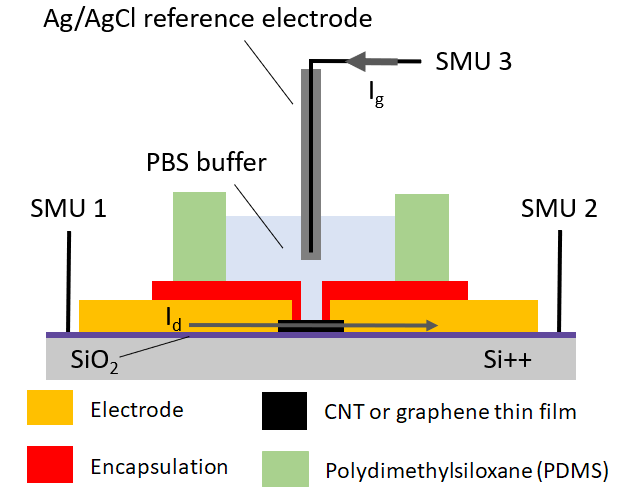
\includegraphics[width=0.9\textwidth,height=\textheight]{./figures/ch4/liquid-gate-schematic.png}

}

\caption{\label{fig-liquid-gate-schematic}Liquid-gated device schematic
showing electrical connections to the three source measure units.
V\(_{\mathrm{ds}}\) is applied between the source SMU (SMU 1) and the
drain SMU (SMU 2), while V\(_{\mathrm{lg}}\) is applied between the gate
SMU (SMU 3) and the drain SMU. The drain SMU is held at 0 V or connected
to a ground plane. Drain current I\(_{\mathrm{d}}\) is measured at the
drain SMU, and gate leakage current I\(_{\mathrm{g}}\) is measured at
the gate SMU.}

\end{figure}

Both back-gated and liquid-gated measurements were taken of carbon
nanotube and graphene devices. Liquid-gated measurements were taken
using the configuration shown in Figure~\ref{fig-liquid-gate-schematic}.
Back-gated measurements were taken with a copper plane placed underneath
the Si/SiO\(_2\) wafer and connected to SMU 3 instead of the reference
electrode.

All measurement setups used had the same basic configuration, with two
source measure units (SMUs) attached to the source and gate. Voltage
from the source and gate SMUs was either kept constant or varied, with
only one SMU varied at a time. Three different measurement setups were
used for taking these measurements, the Agilent (Keysight/HP) 4156C
Semiconductor Parameter Analyser, the Keysight B1500A Semiconductor
Device Analyser, and a National Instruments NI-PXIe modular measurement
system with a 8 GB PXIe-8821 controller and two NI-4138 source measure
units. For measurements with the Keysight instruments, a third, drain
SMU was attached and kept at a constant 0 V (as shown in
Figure~\ref{fig-liquid-gate-schematic}).

\begin{figure}

\begin{minipage}[t]{0.25\linewidth}

{\centering 

~

}

\end{minipage}%
%
\begin{minipage}[t]{0.50\linewidth}

{\centering 

\raisebox{-\height}{

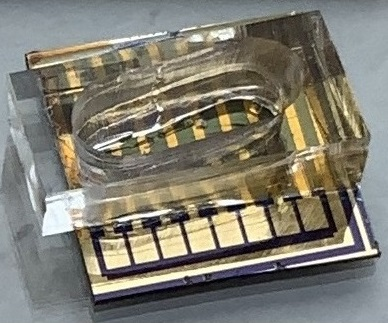
\includegraphics{./figures/ch4/IMG_0845_3.jpg}

}

}

\subcaption{\label{fig-PDMS-device-photo}}
\end{minipage}%
%
\begin{minipage}[t]{0.25\linewidth}

{\centering 

~

}

\end{minipage}%
\newline
\begin{minipage}[t]{0.47\linewidth}

{\centering 

\raisebox{-\height}{

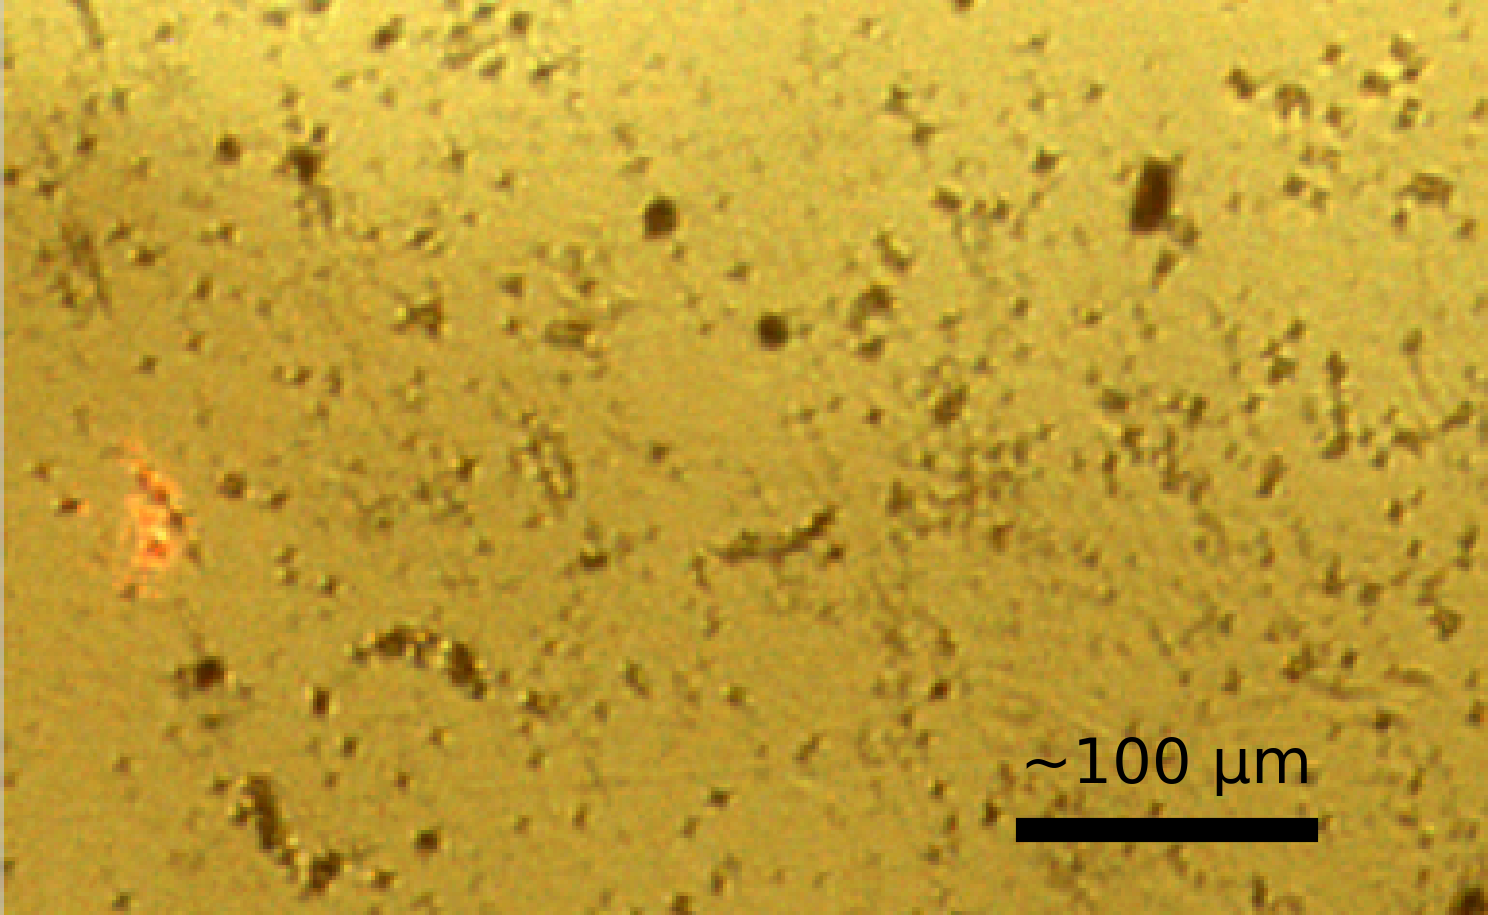
\includegraphics{./figures/ch4/PDMS_dirty.png}

}

}

\subcaption{\label{fig-PDMS_dirty}}
\end{minipage}%
%
\begin{minipage}[t]{0.05\linewidth}

{\centering 

~

}

\end{minipage}%
%
\begin{minipage}[t]{0.47\linewidth}

{\centering 

\raisebox{-\height}{

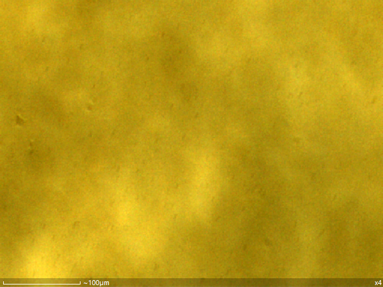
\includegraphics{./figures/ch4/PDMS_clean.png}

}

}

\subcaption{\label{fig-PDMS_clean}}
\end{minipage}%

\caption{\label{fig-PDMS-clean}A carbon nanotube field-effect transistor
device with a polydimethylsiloxane (PDMS) `well' placed on the device
surface is seen in (a), followed by microscope images of the surface of
a well before (b) and after (c) isopropanol (IPA) sonication for 10
minutes.}

\end{figure}

When using the Agilent 4156C Semiconductor Parameter Analyser or
Keysight B1500A Semiconductor Device Analyser for liquid-gated
measurements, a Rucker and Kolls with micromanipulators was used to
contact the devices; when using the National Instruments NI-PXIe for
liquid-gated measurements, a custom-made chip carrier with
spring-loaded, pointed-tip, gold-coated pogo pins was used. Ag/AgCl
standard electrodes were used as the liquid-gate electrode. The
electrode was submerged in 80 \(\mu\)L of PBS buffer in a
polydimethylsiloxane (PDMS) `well' \(-\) a flexible structure used to
contain the electrolyte solution \(-\) with outer dimensions of 12 mm
\(\times\) 6 mm \(\times\) 6 mm. This PDMS well was sonicated in
isopropanol for 10 min and thoroughly N\(_2\) dried before use. The
microscope images seen in Figure~\ref{fig-PDMS-clean} show the PDMS
surface before and after this cleaning step. The end of Ag/AgCl standard
electrode to be submerged should be rinsed in DI water and left to sit
in DI water for 15 minutes before characterisation is performed.

The Agilent 4156C Semiconductor Parameter Analyser and Keysight B1500A
Semiconductor Device Analyser were also used for back-gated measurements
of devices within the vapour delivery system device chamber. When the
lid of this chamber was tightly sealed, it acted a Faraday cage for
another custom-made chip carrier with spring-loaded gold-coated pogo
pins, able to contact four channel electrode pairs at once. The silicon
back of the device was pressed by the pins against a copper block,
connected to the gate SMU.

Custom programs for National Instruments LabView 2017 were used for
measurements from the Agilent 4156C Semiconductor Parameter Analyser and
the National Instruments NI-PXIe. Keysight EasyEXPERT software was used
for characterisation with the Keysight B1500A Semiconductor Device
Analyser.

Liquid-gated transfer characteristics of carbon nanotube FETs were
measured at V\(_{\mathrm{ds}}\) = 100 mV and liquid-gated transfer
characteristics of graphene FETs were measured at V\(_{\mathrm{ds}}\) =
1 V, where V\(_{\mathrm{lg}}\) was swept between -0.5 V and 1 V in both
the forward and reverse direction with a step size of either 10 or 20
mV. Backgated transfer characteristics of carbon nanotube FETs were
either measured at V\(_{\mathrm{ds}}\) = 100 mV or V\(_{\mathrm{ds}}\) =
1 V, where V\(_{\mathrm{bg}}\) was swept between -5 V and 5 V or -10 V
and 10 V in the forward and reverse directions with a step size of 50 mV
or 100 mV.

\hypertarget{sensing-measurements}{%
\subsection{Sensing Measurements}\label{sensing-measurements}}

A liquid-gated setup was used for aqueous-phase sensing and a back-gated
setup in the vapour delivery system was used for vapour-phase sensing,
as described above.

Sensing measurements were performed with constant source-drain and gate
voltages. The gate voltage used was chosen by locating the subthreshold
region of the device transfer characteristics and choosing a voltage
that fell within this region, usually V\(_{\mathrm{g}}\) = 0 V.

Using the NI-PXIe with the PXIe-2737 module, eight-channel multiplexed
current measurements could be taken in rapid succession. An integration
time of 200 or 400 ms was used for sampling with each channel, with the
actual sampling rate set by the NI-PXIe. In practice this meant a
sampling rate of 1.81 s (for 200 ms integration time) or 3.41 s (for 400
ms integration time) for any given channel. A 200 ms integration time
meant the time between samples from successive channels varied between
\(220 ms-230\) ms, while a 400 ms integration time meant the time
between samples was consistently 426 ms. The Keysight equipment used a
constant 1 s sampling interval.

\hypertarget{aqueous-sensing}{%
\subsubsection*{Aqueous Sensing}\label{aqueous-sensing}}
\addcontentsline{toc}{subsubsection}{Aqueous Sensing}

Before the sensing process, 200 \(\mu\)L of PBS was added to the PDMS
well and 100-120 \(\mu\)L of PBS was removed. This initial step was
performed to wet the sides of the PDMS well, and check that the
attachment of the PDMS well to the device would not unseal when larger
volumes of PBS were added during sensing. Before any sensing
measurement, a transfer characteristic curve was taken of the
liquid-gated device.

From Feburary 2022 onwards, the standard sensing addition series used
comprised of a control series and an analyte sensing series. The initial
amount of buffered electrolyte in the well was 100\(\mu\)L, unless
specified otherwise. The total interval for the control series was 1800
s. Electrolyte additions of 20\(\mu\)L were made at 100 s, 200 s and 300
s, while electrolyte subtractions of 20\(\mu\)L were made at 400 s, 500
s and 600 s. The control series was performed as part of each sensing
experiment to test for unwanted responses to electrolyte and to allow
baseline drift to settle. Immediately after the control series, a
sensing sequence was performed as part of the same continuous
measurement set. An initial electrolyte addition was performed at 2100s,
to confirm no changes occurred during the control series that would
interfere with sensing. Unless specified otherwise, five analyte
additions were then made with a time spacing of 300 s, at 2400 s, 2700
s, 3000 s, 3300 s and 3600 s. The experimental series was set to finish
at 4000 s. The exact timings, analyte concentrations and gate voltage
used in a given sensing sequence are discussed alongside the relevant
experimental results.

\hypertarget{vapour-sensing}{%
\subsubsection*{Vapour Sensing}\label{vapour-sensing}}
\addcontentsline{toc}{subsubsection}{Vapour Sensing}

A variety of vapour sensing sequences were used in this work, which are
discussed in \textbf{?@sec-vapour-sensing-biosensors} in detail.

\hypertarget{summary}{%
\section{Summary}\label{summary}}

A variety of approaches were trialled when depositing a carbon nanotube
network for the fabrication of transistor devices, and the resultant
morphology of these networks are discussed in the next chapter. Standard
photolithographic methods were used to successfully fabricate carbon
nanotube and graphene field effect transistor devices. A range of
photolithography types and electrode/encapsulation materials were
trialled to find the optimal device composition for sensing, also
discussed in the next chapter. Atomic force microscopy, fluorescence
microscopy and a variety of electrical measurement setups were used to
characterise the devices.

\appendix
\addcontentsline{toc}{part}{Appendices}

\hypertarget{sec-python}{%
\chapter{Python Code for Data Analysis}\label{sec-python}}

\hypertarget{code-repository}{%
\section{Code Repository}\label{code-repository}}

The code used for general analysis of field-effect transistor devices in
this thesis was written with Python 3.8.8. Contributors to the code used
include Erica Cassie, Erica Happe, Marissa Dierkes and Leo Browning. The
code is located on GitHub and the research group OneDrive, and is
available on request.

\hypertarget{sec-histogram-analysis}{%
\section{Atomic Force Microscope Histogram
Analysis}\label{sec-histogram-analysis}}

The purpose of this code is to analyse atomic force microscope (AFM)
images of carbon nanotube networks in .xyz format taken using an atomic
force microscope and processed in Gwyddion (see
Section~\ref{sec-afm-characterisation}). It was originally designed by
Erica Happe in Matlab, and adapted by Marissa Dierkes and myself for use
in Python.

\begin{equation}\protect\hypertarget{eq-lin-combo-gaussian}{}{
f(x) = k_1\exp{\Bigg(-\frac{{(x-m_1)}^{2}}{{2s_1}^{2}}\Bigg)} + k_2\exp{\Bigg(-\frac{{(x-m_2)}^{2}}{{2s_2}^{2}}\Bigg)} + ...
}\label{eq-lin-combo-gaussian}\end{equation}

The .xyz data is initially sorted into bins with 0.15 nm size. The bin
with the maximum number of counts is set at 0 nm, as this peak
represents the mean of the surface roughness of the bare silicon. The
parameters \(m_i\), \(s_i\), \(k_i\) (i = 1, 2, 3) are used with
objective function Equation~\ref{eq-lin-combo-gaussian} to overlay the
data with normal distributions. These fitting parameters represent the
mean (m), standard deviation (s) and amplitude (k) of each normal
distribution. We can make approximations of some of these fitting
parameters using the histogram data.

\(k_1\) is taken to be the maximum y-value of the data being fitted,
\(m_1\) is set to zero (used as a point of reference) and \(s_1\) is
taken as one-third of the difference between \(m_1\) and the x-value of
the first datapoint where the y-value is greater than 1\% of \(k_1\)
(approximating one standard deviation). We find the distribution given
by these values using Equation~\ref{eq-lin-combo-gaussian}, and subtract
it from the existing dataset.

Then, using the analysis technique outlined by Vobornik \emph{et al.}
\autocite{Vobornik2023} in Gwyddion, we manually find estimates for the
mean \(m_2\) and standard deviation \(s_2\) of the carbon nanotube
bundle distribution. We then take \(k_2\) to be the maximum y-value of
this modified dataset, and \(m_1\) to be the x-value of the maximum
y-value. We then set \(k_2\) so that the height of the resulting
distribution at one standard deviation matches the height of the .xyz
data histogram. We take this distribution, and subtract it from the
existing dataset.

The code also allows for discretely binning continuous data from fitted
normal distributions and examining the proportion of counts above or
below a particular height. 2.9 nm is roughly where 2 bundles with
average size 1.45 nm can start to be present, and is used as an estimate
of the boundary value between single-tube bundle diameters and
multi-tube bundle diameters.

\hypertarget{sec-field-effect-transistor-analysis}{%
\section{Field-Effect Transistor
Analysis}\label{sec-field-effect-transistor-analysis}}

The purpose of this code is to analyse electrical measurements taken of
field-effect transistor (FET) devices. Electrical measurements were
either taken from the Keysight 4156C Semiconductor Parameter Analyser,
National Instruments NI-PXIe or Keysight B1500A Semiconductor Device
Analyser as discussed in Section~\ref{sec-electrical-characterisation};
the code is able to analyse data taken from all three measurement
setups. The main Python file in the code base consists of three related
but independent modules: the first analyses and plots sensing data from
the FET devices, the second analyses and plots transfer characteristics
from channels across a device, and the third compares individual channel
characteristics before and after a modification or after each of several
modifications. The code base also features a separate config file and
style sheet which govern the behaviour of the main code. The code base
was designed collaboratively by myself and Erica Cassie over GitHub
using the Sourcetree Git GUI.

The first of the three modules is for processing sensing datasets. This
module imports sensing measurements in .csv format and analyses them,
then outputs a plot of the raw data, alongside multiple plots which have
been modified in various ways. It can also fit exponential and linear
trendlines to regions of the sensing data, as well as find the signal
change per analyte addition, and returns spreadsheets containing the
results of these analyses. These spreadsheets include the standard
deviation for all included parameters. Modified plots include normalised
plots (type of normalisation can be set in config file), plots with
fitted curves, plots with the linear baseline drift removed, plots of
signal with analyte addition, ``despiked'' plots and ``filtered'' plots.
It is possible to add annotations to any of these plots using the config
file, and it is possible to produce a plot with a combination of these
modifications.

The scipy.optimize.curve\_fit module is used to fit linear and
exponential curves to regions of interest of the sensing data. Initial
parameters for the scipy.optimize.curve\_fit module are chosen by
approximating fitting parameters in a similar manner to the approach in
Section~\ref{sec-histogram-analysis}. For a linear fit \(mt + b\), the
parameters are simply set as \(m=1\) and \(b=0\). For an exponential fit
\(a\exp{(-t/\tau)} + c\), \(c\) is set as the final current measurement
of the region of interest and \(a\) is set as the initial current
measurement minus \(c\). Then, \(\tau\) is set as the time where current
has dropped to \(e^{-1}a + c\).

``Despiked'' plots have had spurious datapoints removed through the use
of an interquartile range rolling filter. The window size of the rolling
filter used was 40 datapoints, and datapoints in each window with a
z-score above \(\pm 3\) were removed from the plotted/processed data.
``Filtered'' plots had noise reduced using a moving median filter. The
moving median filter is more effective at removing noise than a simple
moving average, and has advantages over other filters (such as the
Savitzky-Golay filter) when removing noise from data with sharp edges,
as is the case for sensing data. Median filtering can also be used for
baseline drift compensation, though this approach was not used in this
thesis \autocite{Stone2011}. The moving median filter used had a window
of 40 datapoints.

Plots of signal with analyte addition were constructed from current data
after first removing baseline drift and applying a moving median filter.
A simple difference calculation between the mean of the filtered current
before an addition and the mean of the filtered current after the
addition was performed at each addition. These differences were then
normalised relative to the initial current. The signal with analyte
addition give reasonably consistent results regardless of whether
baseline drift was removed from the data, as shown in
Figure~\ref{fig-spaa-plot-comparison}. We can therefore be confident
that robust signal with analyte addition plots are robust even in the
presence of significant drift.

\begin{figure}

\begin{minipage}[t]{0.50\linewidth}

{\centering 

\raisebox{-\height}{

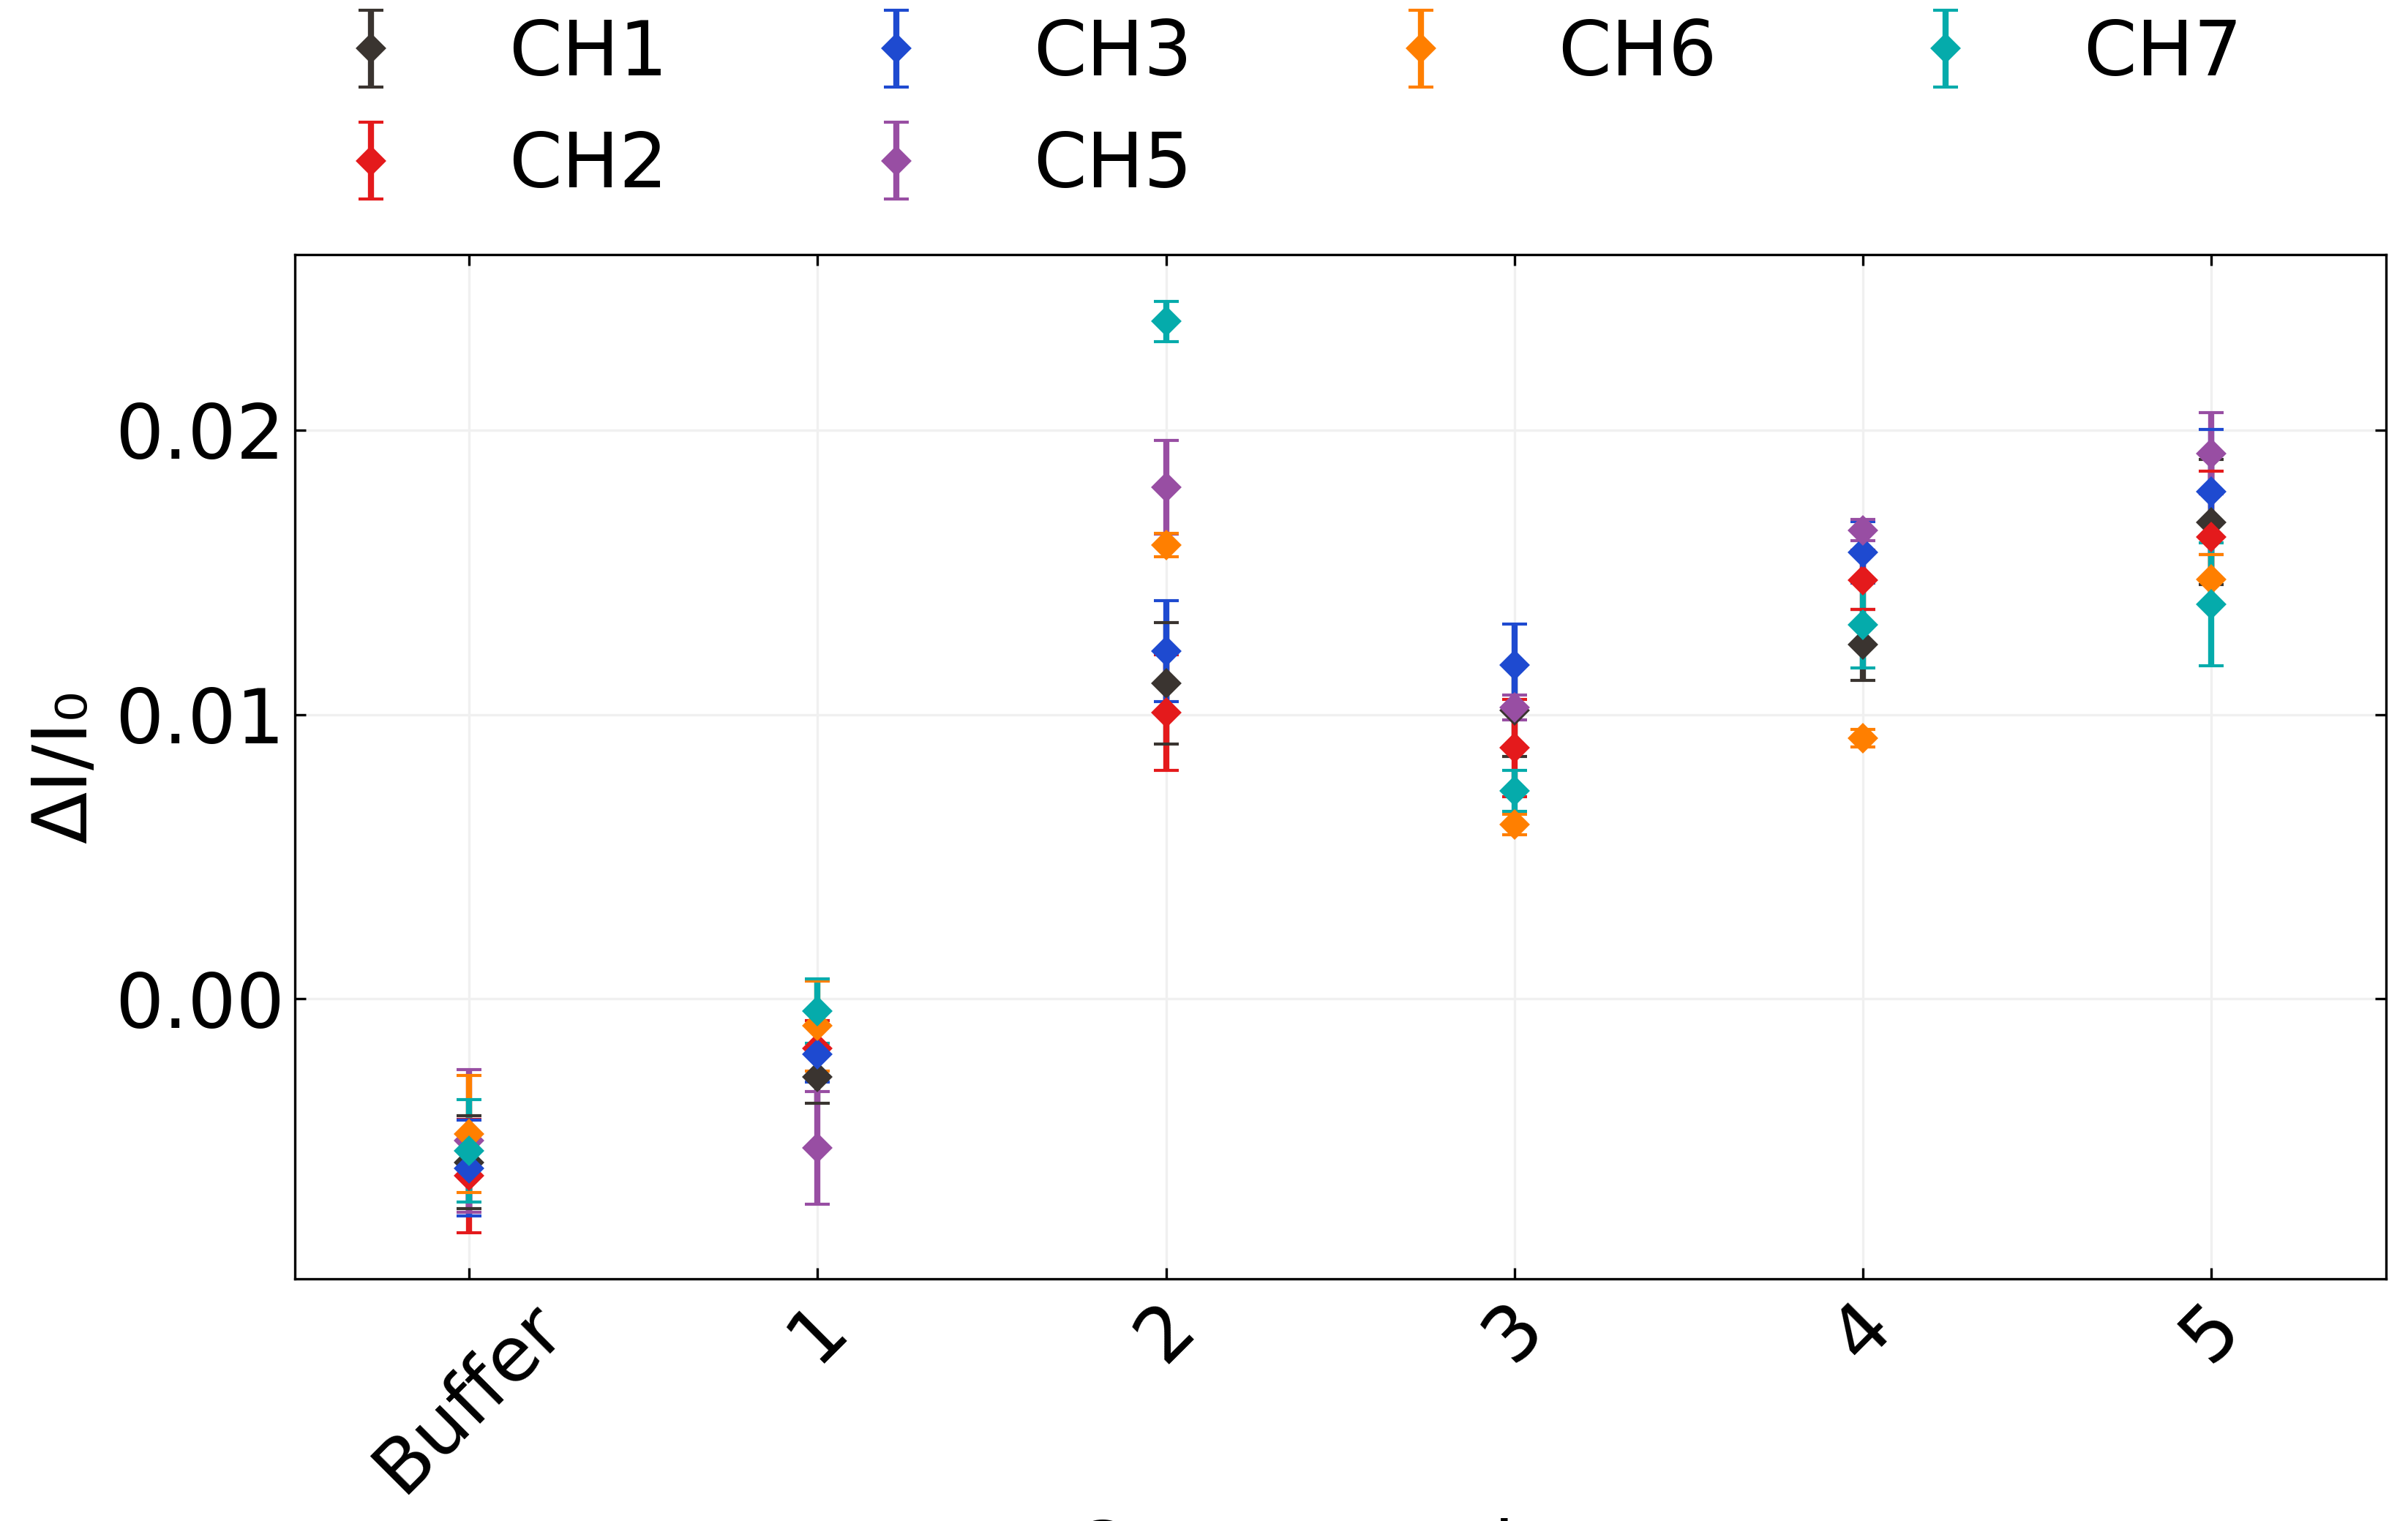
\includegraphics{./figures/app1/NTQ31C1_mean_simple_difference_before_and_after_step_filtered_concentrations.png}

}

}

\subcaption{\label{fig-spaa-no-detrend}}
\end{minipage}%
%
\begin{minipage}[t]{0.50\linewidth}

{\centering 

\raisebox{-\height}{

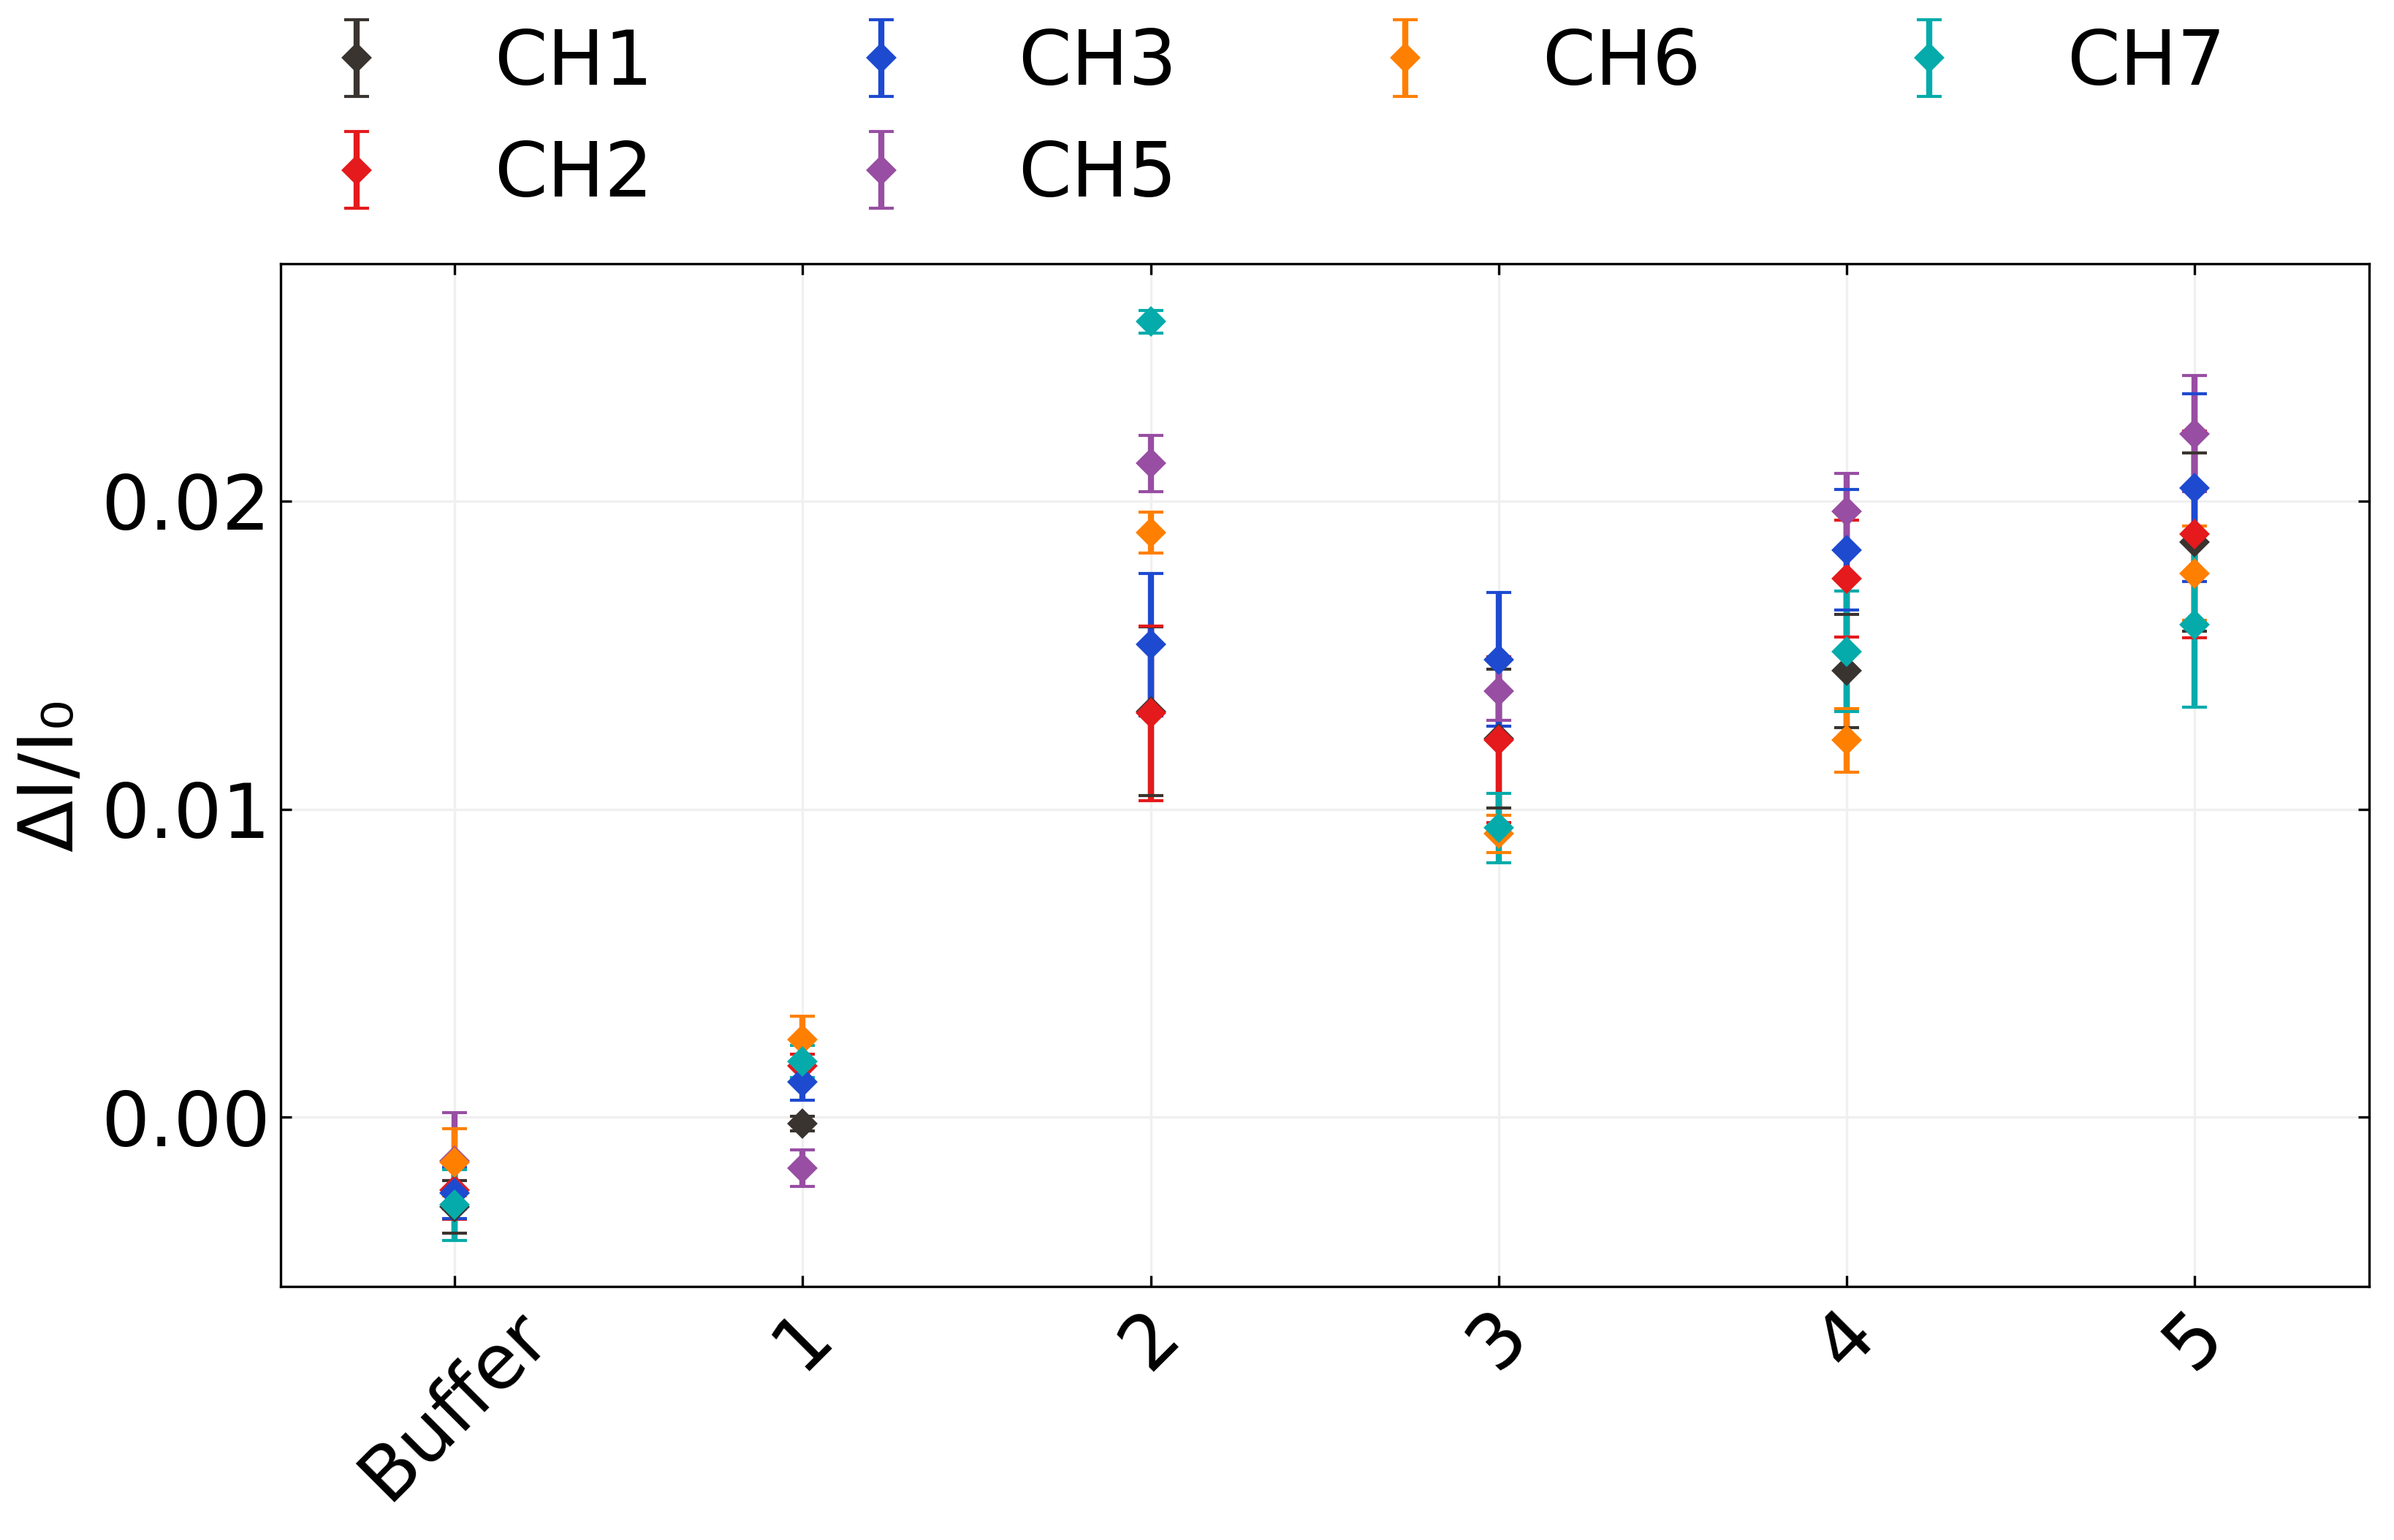
\includegraphics{./figures/app1/NTQ31C1_mean_simple_difference_before_and_after_step_filtered_concentrations_detrend.png}

}

}

\subcaption{\label{fig-spaa-detrend}}
\end{minipage}%

\caption{\label{fig-spaa-plot-comparison}A comparison of signal with
analyte addition plots taken from the same salt concentration sensing
dataset (the same dataset as used in \textbf{?@fig-salt-conc-sensing}).
In (a), a simple difference calculation performed on filtered data was
used, while in (b) the same calculation was performed on filtered data
with the baseline drift removed, the method used in the body of the
thesis.}

\end{figure}

The second module imports transfer measurements in .csv format and
creates combined and individual plots of the eight channels on a single
device. In combined plots, channels which are non-working, due to being
shorted or non-conducting, are removed via setting a maximum and minimum
possible on-current in the config file. Various parameters from the
transfer characteristics are saved as a spreadsheet along with standard
error. These parameters include on current, off current, subthreshold
slope and threshold voltage for the carbon nanotube devices, and on
current, off current and major Dirac point voltage for graphene devices.
The device type being analysed can be set in the config file.

The third module imports several transfer measurements in .csv format
and allows for comparison of the same channel before and after some
modification. It also calculates the shift in either threshold voltage
or major Dirac voltage of the device.

\hypertarget{vapour-delivery-system}{%
\chapter{Vapour Delivery System}\label{vapour-delivery-system}}

\hypertarget{technical-notes}{%
\section{Technical Notes}\label{technical-notes}}

Two LabView Virtual Instruments (VIs) were adapted from pre-existing VIs
for operating the mass flow controllers and monitoring vapour flow into
the device chamber, as well as monitoring temperature and humidity in
the vapour delivery system's manifold. These VIs were named ``\,'' A
third VI was developed in parallel which combined the first two Virtual
Instruments, alongside allowing the sequence of values to control the
mass flow controllers.

From Honours report: ``\,``\,'' Figure 12 gives the right side of the
front panel of the LabView VI sample with vapour.VI, which letsus preset
an autonomously-performed vapour sensing sequence. Each row in each
array module corresponds to a differennest step in this sequence. The
`howManySteps' module lets us set how many of these steps are performed.
The `Durations Array' module determines the length of time in seconds
each step is performed over. The `Carrier Flows Array' and `Dilution
Flows Array' modules let us set the carrier flow and dilution flow,
respectively, in standard cubic centimetres per minute (sccm) through
the gas rig at each step. The carrier flow pushes analyte vapour into
the vapour-sensing device chamber, while dilution flow is used to modify
the flow behaviour of the analyte vapour entering the chamber. The
vapour sensing sequence as depicted in Figure 12 was used for all vapour
sensing runs in this investigation. At the end of the sequence, the data
collected about the vapour sensing process was saved as an .lvm file.
``\,``\,''

\hypertarget{future-improvements}{%
\section{Future Improvements}\label{future-improvements}}


\backmatter
\printbibliography


\end{document}
